\documentclass[onecolumn]{IEEEtran}

\usepackage[utf8]{inputenc}
\usepackage[T1]{fontenc}
\usepackage{mathtools}
\usepackage{amssymb}
\usepackage{amsmath}

\numberwithin{equation}{section}
\DeclareMathOperator*{\argmax}{arg\,max}
\DeclareMathOperator*{\argmin}{arg\,min}
\DeclareMathOperator{\diag}{diag}

\usepackage{amsthm}
\usepackage{thmtools}

\newtheorem{theorem}{Theorem}[section]
\newtheorem{lemma}[theorem]{Lemma}
\newtheorem{corollary}[theorem]{Corollary}
\newtheorem{proposition}[theorem]{Proposition}

\theoremstyle{definition}
\newtheorem{definition}[theorem]{Definition}
\newtheorem{example}[theorem]{Example}

\theoremstyle{remark}
\newtheorem{remark}[theorem]{Remark}
\newtheorem*{note}{Note}

\usepackage{booktabs}
\usepackage{array}
\usepackage{multirow}
\usepackage{tabularx}
\usepackage{longtable}
\usepackage{siunitx}

\newcolumntype{C}[1]{>{\centering\arraybackslash}p{#1}}
\newcolumntype{L}[1]{>{\raggedright\arraybackslash}p{#1}}
\sisetup{
    table-format = 3.2,
    table-auto-round = true
}

\usepackage{tikz}
\usepackage{pgfplots}
\pgfplotsset{compat=1.18}

\usetikzlibrary{
  arrows.meta,
  positioning,
  shapes.geometric,
  shadows,
  fit,
  calc,
  matrix,
  shapes.misc
}
\tikzset{
  base/.style = {rectangle, rounded corners, draw=black, minimum width=2.5cm, minimum height=1cm, text centered, font=\sffamily},
  startstop/.style = {base, fill=red!20, drop shadow},
  process/.style = {base, fill=blue!20, drop shadow},
  decision/.style = {diamond, aspect=1.5, draw=black, fill=green!20, drop shadow, align=center},
  arrow/.style = {thick, -{Stealth[length=3mm]}},
  matrix_style/.style={matrix of nodes, row sep=0.5cm, column sep=0.5cm, nodes={anchor=center}},
  dashdot/.style={dash pattern=on 3pt off 3pt on 1pt off 3pt}
}

\usepackage{algorithm}
\usepackage{algorithmicx}
\usepackage{algpseudocode}

\algrenewcommand\algorithmicrequire{\textbf{Input:}}
\algrenewcommand\algorithmicensure{\textbf{Output:}}

\usepackage{graphicx}
\usepackage{url}
\usepackage{xcolor}
\usepackage{caption}
\usepackage[colorlinks=true, linkcolor=blue, citecolor=green!50!black, urlcolor=blue!80!black]{hyperref}

\IEEEoverridecommandlockouts

\begin{document}

\title{Verified Localized Episodic Grounding: Robust Memory Consolidation for Large Language Models in Heterogeneous Environments}
\author{}

\maketitle

\begin{abstract}
Large Language Models (LLMs) increasingly rely on in-context episodic memory to solve complex, multi-modal tasks. However, in heterogeneous or non-stationary environments, extracting unified global semantic rules from unstructured episodes often fails due to context-dependent contradictions. While existing localized reflection methods attempt to address this by generating sample-by-sample abstractions, they typically lack rigorous post-generation verification, leading to the accumulation and propagation of hallucinated heuristics. To overcome these limitations, we propose Verified Localized Episodic Grounding (VLEG), a novel memory framework that bridges raw episodic recall and robust semantic abstraction. VLEG introduces an iterative cyclic refinement process at the localized episodic level, employing a strict generate-and-verify loop to prune flawed or logically inconsistent reflections before they are committed to memory. During the inference phase, VLEG utilizes hybrid grounding, conditioning the reasoning module on both the high-dimensional raw episodes and their rigorously verified low-dimensional reflections. This dual approach preserves concrete contextual details while providing a reliable semantic scaffold. In a reduced-order reimplementation designed to test these claims directly (Section~\ref{sec:exp1}--\ref{sec:exp5}), primarily using a 7B-parameter open-weight model, we find a more qualified picture than the framework's motivation suggests: at 7B scale, the simplest possible baseline (raw in-context retrieval with no abstraction) matched or outperformed VLEG at every task level, and hybrid grounding under-performed both raw episodic retrieval and abstraction-only retrieval specifically on the heterogeneous, masked-combination condition it was intended for. Repeating all five experiments with a 70B-parameter model resolved these differently: the baseline comparison reversed cleanly (VLEG matched or beat the same baseline at every level tested across three independent seeds), the hybrid-grounding comparison resolved only partially (Hybrid Grounding tied for best overall accuracy at 70B, but Abstract-Only retrieval retained a narrower edge specifically on masked combinations, in the same direction as the 7B result), and a separate parameter-sensitivity check found a genuine performance plateau in refinement iterations that became sharper and fully reproducible at 70B, one iteration earlier than originally claimed. Separately, iterative verification reliably improves memory coverage and downstream accuracy over an unverified single-step baseline, an effect that held and strengthened at both model scales, but a per-episode verifier is structurally unable to detect over-specified or spuriously-attributed reflections relative to an unverified baseline — a finding that held unchanged across both model scales even as the raw rate of such errors fell sharply with the larger model. We report these results, including where they diverge from the framework's original motivating hypotheses and where they resolve differently at different model scales, alongside the conditions under which VLEG's components do help.
\end{abstract}

\begin{IEEEkeywords}
Large Language Models, Episodic Memory, Semantic Abstraction, In-Context Learning, Hallucination Mitigation, Hybrid Grounding, Iterative Refinement
\end{IEEEkeywords}


\section{Introduction}

\subsection{Background: In-Context Learning and Memory Augmentation}

The foundational capabilities of modern Large Language Models (LLMs) are heavily anchored in the paradigm of In-Context Learning (ICL), as introduced by Brown et al. \cite{brown2020language}. In this framework, the prompt context effectively functions as a form of short-term working memory. By providing a few raw episodic examples within the prompt, LLMs can dynamically adapt to and perform novel tasks without requiring any gradient-based parameter updates. While ICL has revolutionized zero-shot and few-shot generalization, its reliance on a strictly finite context window inherently limits its scalability. As the complexity and volume of the provided examples increase, the model's ability to effectively attend to relevant information degrades, leading to cognitive overload and diminished reasoning performance.

To address the limitations of transient working memory, the development of AI agents has increasingly focused on the integration of persistent memory structures. This evolution is driven by the need to support long-horizon planning, continuous learning, and complex reasoning in dynamic environments. Recent comprehensive surveys on LLM memory mechanisms \cite{wu2025from, zhang2024survey} detail this trajectory, highlighting a broader academic quest to equip artificial agents with human-like cognitive architectures. These architectures aim to transition LLMs from stateless text generators into stateful entities capable of accumulating, organizing, and leveraging vast repositories of historical interactions over time.

Historically, the dominant approach to implementing persistent memory has been passive, retrieval-based systems, most notably Retrieval-Augmented Generation (RAG) \cite{lewis2020retrieval}. RAG equips LLMs with a long-term datastore from which relevant raw episodes or text chunks are dynamically retrieved and injected into the context window at inference time. However, this passive mechanism merely shifts the computational bottleneck from storage capacity to inference-time reasoning. By relying exclusively on the retrieval of unstructured, raw data, passive systems force the LLM to perform ad-hoc abstraction over a noisy sea of information on the fly. Recognizing this critical inefficiency, the frontier of memory augmentation has shifted toward active memory consolidation—systems that actively distill, verify, and abstract raw experiences into structured semantic knowledge prior to inference. This transition from passive episodic recall to active semantic abstraction sets the necessary stage for addressing the fundamental trade-offs in memory-augmented reasoning.

\subsection{Problem Definition: The Limits of Global Abstraction and Unverified Local Reflection}

Despite the theoretical appeal of utilizing the prompt context as a short-term working memory, Large Language Models (LLMs) exhibit fundamental limitations when forced to reason directly over raw, unstructured episodic data. As the complexity and dimensionality of multi-modal experiences increase, the sheer volume of high-fidelity details rapidly overwhelms the effective context window. Consequently, LLMs suffer a significant degradation in reasoning performance, failing to autonomously distill latent rules from a noisy sea of raw episodic memories \cite{an2024why}. 

To mitigate the cognitive overload associated with pure episodic retention, recent methodologies have introduced localized reflection mechanisms. Frameworks such as Reflexion \cite{shinn2023reflexion} and Voyager \cite{wang2024voyager} process experiences on a sample-by-sample basis, generating localized summaries or procedural critiques to guide future actions. However, these approaches predominantly rely on single-step or unverified multi-step linear generation pipelines. Because they lack a rigorous, closed-loop verification mechanism to validate the generated reflections against the original raw evidence, these systems are highly susceptible to semantic drift. Over time, they inevitably accumulate hallucinated or logically flawed heuristics, which subsequently corrupt the agent's reasoning capabilities when retrieved for novel tasks.

Conversely, state-of-the-art memory augmentation has shifted toward global semantic consolidation, aiming to synthesize information across multiple disparate episodes to induce overarching abstract rules. Methods such as Hypothesis-Driven Reasoning (HDR) \cite{agarwal2026hypothesis} and IDEA \cite{he2024idea} attempt to distill a single, unified set of global hypotheses from the entire episodic memory bank. While effective in homogeneous domains, this approach is mathematically ill-posed in highly heterogeneous or non-stationary environments. In complex real-world scenarios, local episodes are frequently governed by mutually exclusive, context-dependent heuristics. When forced to extract a universal consensus from such contradictory data, global semantic models either collapse into semantic over-abstraction—generating overly generic statements that lose critical conditional logic—or hallucinate false global rules that fail catastrophically on edge cases. Thus, a critical gap remains: how to achieve reliable semantic generalization without falling victim to the unverified noise of local reflections or the over-abstraction of global hypotheses.

\subsection{Our Contribution: Verified Localized Episodic Grounding (VLEG)}

To resolve the fundamental contradiction between retaining high-fidelity episodic detail and achieving robust semantic generalization, we propose a novel framework: Verified Localized Episodic Grounding (VLEG). VLEG is specifically designed to operate in highly heterogeneous and non-stationary environments where global rule extraction fails. Instead of forcing a unified global consensus that risks over-abstraction, VLEG shifts the abstraction target to the localized episode, ensuring that context-dependent heuristics are preserved and explicitly grounded in their originating multi-modal experiences.

The core memory consolidation mechanism of VLEG relies on the application of \textit{Iterative Cyclic Refinement} at the localized episodic level. Unlike prior localized memory systems that utilize single-step generation or unverified linear pipelines \cite{shinn2023reflexion, zhong2024memorybank}, VLEG enforces a strict, closed-loop generate-and-verify architecture. For every raw episode, a candidate reflection is generated and subsequently evaluated by an independent, strict verifier against the raw episodic evidence. If a logical inconsistency or hallucination is detected, the verifier issues a critique, prompting the generator to refine the reflection. This cycle continues until the reflection is explicitly validated. This verification loop bounds the probability of committing a reflection whose stated conclusion contradicts the episode it was generated from; Section~\ref{sec:vleg-methodology} and Experiment 5 (Section~\ref{sec:exp5}) discuss why this guarantee does not extend to reflections that reach the right conclusion via an over-specified or spuriously-attributed justification, which we find is the more common failure mode in practice.

Furthermore, to effectively leverage these verified local abstractions during downstream reasoning, VLEG introduces a \textit{Hybrid Grounding} inference strategy. When presented with a novel target task, the system retrieves the most relevant memory tuples and conditions the reasoning Large Language Model (LLM) simultaneously on both the raw, high-dimensional episodic data and its corresponding rigorously verified, low-dimensional reflection. This dual-pathway integration ensures that the model benefits from the cognitive scaffold of abstract logical rules without losing the concrete visual or textual details necessary for complex, context-dependent disambiguation. This approach stands in stark contrast to pure episodic retrieval methods that overwhelm the context window with unstructured noise \cite{purohit2025sample}, as well as pure semantic application strategies that risk catastrophic reasoning failures due to semantic over-abstraction \cite{li2024memory}.

\subsection{Paper Organization}

The remainder of this paper is organized as follows. Section 2 reviews the related literature, focusing on the evolution of memory abstraction paradigms and recent advancements in hypothesis generation \cite{zhou2024hypothesis, qiu2024phenomenal}. Section 3 provides a comprehensive exposition of the Verified Localized Episodic Grounding (VLEG) methodology. This includes the formalization of the localized memory consolidator, the multi-agent strict verifier architecture, and the hybrid inference integration strategy. Section 4 outlines our rigorous experimental design, introducing the heterogeneous Experience-Transfer tasks of varying complexities. Finally, Section 5 presents the empirical results, offering a detailed analysis of task accuracy, memory quality diagnostics, and computational overhead, before concluding with a discussion on the framework's limitations and promising directions for future research.
\section{Related Work}

\subsection{Pure Episodic Retention and Direct Retrieval}

The most fundamental paradigm in memory-augmented Large Language Models (LLMs) relies on Pure Episodic Retention, wherein the system stores raw, unmodified multi-modal or textual experiences. Within our proposed MECE framework, these methodologies are characterized by Single-Step Direct Generation (as no active abstraction occurs prior to inference) and Episodic-Only Retrieval (where the model is conditioned exclusively on raw historical samples). 

The foundational instantiation of this approach is In-Context Learning (ICL), introduced by Brown et al. \cite{brown2020language}. ICL demonstrated that LLMs can adapt to novel tasks simply by being provided with a few raw episodic examples in their prompt context, effectively utilizing the context window as a short-term working memory. While ICL preserves the high-fidelity details of each episode, its reliance on unstructured data severely limits its scalability. To address the inherent constraints of the context window, Lewis et al. \cite{lewis2020retrieval} introduced Retrieval-Augmented Generation (RAG). RAG equips the LLM with a passive, long-term episodic datastore, dynamically retrieving the most relevant raw episodes at inference time. 

Subsequent research within this paradigm has focused heavily on optimizing the retrieval and selection mechanisms to maximize the utility of the retrieved episodes. For instance, Zhang et al. \cite{zhang2022active} proposed active retrieval strategies to dynamically select the most informative examples for ICL, while Purohit et al. \cite{purohit2025sample} explored sample-efficient retrieval techniques to minimize context bloat. Despite these optimizations, these approaches remain fundamentally constrained by their lack of an active abstraction mechanism. Because they rely on Single-Step Direct Generation over raw data at test time, the burden of inducing latent rules from a noisy sea of unstructured experiences falls entirely on the inference model's ad-hoc reasoning capabilities.

This architectural reliance on pure episodic data introduces a critical vulnerability. As empirically demonstrated by An et al. \cite{an2024why}, LLMs suffer a significant degradation in reasoning performance as the raw episodes become more complex or heterogeneous. When faced with high-dimensional, multi-modal tasks where local rules may contradict global distributions (such as the masked combinations in our Level 3 Experience-Transfer task), the model becomes overwhelmed by episodic noise and fails to autonomously distill the underlying abstract patterns. 

The shortcomings of Pure Episodic Retention directly highlight the research gaps addressed by our proposed Verified Localized Episodic Grounding (VLEG) framework. The failure of models to process complex raw episodes without hallucination underscores the necessity of moving beyond Episodic-Only Retrieval. By introducing an Iterative Cyclic Refinement pipeline to generate verified local reflections, and subsequently employing Hybrid Grounding during inference, VLEG actively bridges the gap between the high-fidelity noise of pure episodic retention \cite{brown2020language, lewis2020retrieval} and the need for robust, reliable semantic abstraction.

\subsection{Localized Episodic Reflection}

To mitigate the context window exhaustion and noise inherent in pure episodic retention, a subsequent wave of memory augmentation methodologies introduced the concept of Localized Episodic Reflection. Rather than storing raw experiences indefinitely, these approaches process experiences on a sample-by-sample basis, generating localized summaries, procedural critiques, or heuristic insights for individual episodes. While this significantly reduces the raw token count and highlights salient features, the architectural mechanisms used to generate these reflections vary, leading to distinct trade-offs in reliability and reasoning quality.

Early implementations of localized abstraction utilized Single-Step Direct Generation coupled with Episodic-Only Retrieval. For instance, Zhong et al. \cite{zhong2024memorybank} proposed MemoryBank, which generates localized summaries of user interactions in a single forward pass to serve as long-term memory. While computationally inexpensive, this single-step architecture is highly susceptible to hallucination. Because the model is prompted to extract patterns without any intermediate reasoning or verification steps, it frequently generates flawed or overly simplistic heuristics that fail to capture the nuances of complex, multi-modal environments. Furthermore, by relying on Episodic-Only Retrieval during inference, the system treats these unverified summaries as standalone facts, propagating errors into the downstream reasoning tasks.

To address the limitations of single-step generation, more sophisticated frameworks adopted Multi-Step Linear Generation pipelines. A foundational work in this category is Reflexion \cite{shinn2023reflexion}, which allows agents to verbally reflect on individual past episodes through a sequential pipeline of evaluation and critique, thereby identifying mistakes to improve future performance. Similarly, Voyager \cite{wang2024voyager} employs a linear pipeline to distill procedural skills from localized environmental interactions, while recent works like AMEM \cite{xu2025amem} and the framework proposed by Kim et al. \cite{kim2024towards} utilize multi-stage hierarchical summarization to structure localized memories. 

Despite providing more structured reasoning than single-step methods, these multi-step linear pipelines exhibit a critical shortcoming: they operate as open-loop systems. Because the abstraction process is sequential and non-cyclic, there is no mechanism to self-correct or rigorously verify the generated reflections against the raw episodic evidence before committing them to memory. Consequently, hallucinated or logically inconsistent heuristics can still accumulate over time. 

This architectural vulnerability directly highlights the primary research gap addressed by our proposed Verified Localized Episodic Grounding (VLEG) framework. Existing localized reflection methods lack an \textit{Iterative Cyclic Refinement} mechanism at the sample level. By failing to enforce a strict generate-and-verify loop, methods like Reflexion \cite{shinn2023reflexion} and Voyager \cite{wang2024voyager} cannot mathematically bound the probability of hallucination propagation. Furthermore, these frameworks predominantly rely on Episodic-Only Retrieval, fetching the generated reflections in isolation. By contrast, VLEG not only introduces cyclic verification to ensure the validity of local heuristics but also employs \textit{Hybrid Grounding} during inference. This ensures that the reasoning module is conditioned on both the rigorously verified local abstraction and the high-fidelity raw episode, preventing the semantic over-abstraction that plagues current localized memory systems.

\subsection{Global Semantic Consolidation}
\label{sec:related-work-global-consolidation}
To overcome the limitations of localized reflection and pure episodic retention, a growing body of literature has focused on \textit{Global Semantic Consolidation}. Methodologies in this category actively synthesize information across multiple disparate episodes to induce abstract, global rules or hypotheses. By distilling a noisy sea of unstructured experiences into a concise semantic memory, these approaches aim to minimize context window noise and maximize zero-shot generalization on novel tasks. The evolution of this paradigm can be traced through the increasing sophistication of its abstraction pipeline architectures.

The earliest approaches to global semantic consolidation relied on \textit{Single-Step Direct Generation}. For instance, \cite{he2024idea} proposed the IDEA framework, which prompts Large Language Models (LLMs) to perform induction, deduction, and abduction in a single forward pass to generate overarching hypotheses from text-based episodes. While computationally inexpensive and effective in low-complexity text domains, single-step generation is highly susceptible to hallucination. When applied to high-dimensional, multi-modal environments, these models frequently fail to autonomously distill accurate latent rules, as a single prompt is insufficient to disentangle complex, overlapping features without intermediate reasoning steps.

To mitigate the hallucination risks of single-step methods, subsequent research introduced \textit{Multi-Step Linear Generation} pipelines. These frameworks divide the abstraction process into sequential, non-cyclic stages, such as hierarchical summarization or chain-of-thought factor extraction. Several works, including \cite{lee2024generating, kim2023machine, li2024memory}, successfully implemented multi-step linear pipelines to construct robust global rules. However, these systems predominantly utilize a \textit{Semantic-Only Application} strategy during inference. By providing the inference model solely with the distilled global hypotheses, they entirely eliminate episodic noise but simultaneously deprive the model of concrete grounding examples. This creates a critical vulnerability: if the generated semantic rules are overly abstract, slightly inaccurate, or fail to capture edge cases, the model has no raw evidence to fall back on, leading to catastrophic reasoning failures. Addressing this integration flaw, \cite{wang2025mirix} advanced the linear pipeline paradigm by incorporating \textit{Hybrid Grounding}, allowing the model to reference both the linearly generated global rules and a subset of raw episodes at test time. 

Despite the improvements in inference integration, multi-step linear pipelines still lack a mechanism to self-correct flawed abstractions during the memory generation phase itself. This limitation spurred the development of \textit{Iterative Cyclic Refinement} architectures. Works such as \cite{qiu2024phenomenal} and \cite{zhou2024hypothesis} employ closed-loop generate-and-verify systems, where global hypotheses are iteratively proposed, tested against the episodic memory bank, and refined or pruned. While these cyclic frameworks maximize the semantic accuracy of the generated rules, they largely remain confined to Semantic-Only Application, again risking over-abstraction at inference time.

More fundamentally, all of the aforementioned global semantic consolidation frameworks share a critical theoretical shortcoming that directly motivates our research gap: they operate on the assumption that a single, unified set of global rules can be successfully distilled from the entire episodic memory. In highly heterogeneous, non-stationary, or masked environments (such as our Level 3 Experience-Transfer tasks), global rule extraction becomes mathematically ill-posed because local episodes may be governed by mutually exclusive, context-dependent heuristics. When global abstraction fails, these systems either collapse into generating overly generic statements or enter infinite refinement loops. This fundamental limitation underscores the necessity of shifting the rigorous generate-and-verify loop away from global consolidation and applying it at the localized level, as proposed in our Verified Localized Episodic Grounding (VLEG) framework.

\subsection{Hybrid Episodic-Semantic Grounding}

The integration strategy employed during the inference phase dictates how a Large Language Model (LLM) balances high-fidelity contextual details against generalized reasoning heuristics. Recent comprehensive surveys on LLM memory mechanisms, such as those by Wu et al. \cite{wu2025from} and Zhang et al. \cite{zhang2024survey}, emphasize that human-like cognitive architectures rely on a dual-pathway retrieval system. Relying solely on episodic retrieval risks overwhelming the context window with unstructured noise, whereas semantic-only application deprives the model of necessary grounding, frequently leading to hallucination via over-abstraction. Hybrid Episodic-Semantic Grounding addresses this dichotomy by conditioning the inference model simultaneously on raw episodic data and distilled semantic rules.

The state-of-the-art in this domain is exemplified by the Hypothesis-Driven Reasoning (HDR) framework \cite{agarwal2026hypothesis}. HDR occupies a highly sophisticated and relatively sparse region of the methodological solution space, uniquely combining Global Semantic Consolidation, Iterative Cyclic Refinement, and Hybrid Grounding. During the inference phase on a novel task, HDR retrieves both the raw multi-modal episodes and the globally verified hypotheses. This dual-pathway integration allows the LLM to leverage abstract rules for global guidance while retaining the raw episodes for concrete visual or textual grounding, effectively bridging the gap between inductive rule learning and deductive application \cite{agarwal2026hypothesis}.

Despite its empirical success and robust architectural design, the reliance of HDR \cite{agarwal2026hypothesis} on \textit{Global} Semantic Consolidation introduces a critical vulnerability. By attempting to distill a single, unified set of global rules from the entire episodic memory bank, HDR implicitly assumes a homogeneous underlying data distribution. In highly heterogeneous or non-stationary environments, local episodes are frequently governed by mutually exclusive, context-dependent heuristics. Under such conditions, global rule extraction becomes mathematically ill-posed; the iterative refinement loop is forced to either discard valid local rules (treating them as anomalies) or converge on overly generic, unhelpful hypotheses that fail to provide meaningful semantic guidance.

This fundamental limitation directly motivates the primary research gap addressed in this work. While the broader literature \cite{wu2025from, zhang2024survey} strongly advocates for hybrid memory structures, existing methodologies have yet to explore Hybrid Grounding coupled with \textit{Localized} Episodic Reflection and Iterative Cyclic Refinement. By shifting the semantic abstraction from a global corpus-level to a localized episode-level, and rigorously verifying these local reflections before hybrid inference, our proposed Verified Localized Episodic Grounding (VLEG) framework resolves the shortcomings of global abstraction. VLEG preserves the concrete contextual details of the raw episode while providing a robust, context-specific semantic scaffold that remains stable even under extreme global heterogeneity.
\section{The Proposed Method}
\label{sec:vleg-methodology}

\subsection{Overview of Verified Localized Episodic Grounding (VLEG)}
The Verified Localized Episodic Grounding (VLEG) framework is designed to address the fundamental limitations of existing memory augmentation paradigms when deployed in highly heterogeneous, non-stationary environments. Current approaches to Large Language Model (LLM) memory generally fall into two extreme categories: pure episodic retention and global semantic consolidation. VLEG introduces a principled middle ground, leveraging the strengths of both paradigms while mathematically bounding the propagation of hallucinated heuristics.

To formalize the problem space, let $\mathcal{E} = \{e_1, e_2, \dots, e_n\}$ represent a stream of multi-modal episodic experiences encountered by an agent. In the paradigm of pure episodic retention \cite{brown2020language}, the memory bank is simply the identity mapping of the experience stream, $\mathcal{M}_{ep} = \mathcal{E}$. While this preserves high-fidelity contextual details, reasoning directly over $\mathcal{M}_{ep}$ during inference imposes an overwhelming cognitive load on the LLM, often exceeding effective context window limits and leading to degraded reasoning performance due to noise.

Conversely, global semantic consolidation \cite{agarwal2026hypothesis} attempts to distill $\mathcal{E}$ into a compact set of universal rules or hypotheses, $\mathcal{H}$. This can be modeled as finding a global hypothesis set that maximizes the likelihood of the observed episodes:
\begin{equation}
    \mathcal{H}^* = \arg\max_{\mathcal{H}} P(\mathcal{H} \mid e_1, e_2, \dots, e_n)
\end{equation}
However, in highly heterogeneous environments, the underlying data distribution is not governed by a single, unified set of rules. Instead, local episodes may be governed by mutually exclusive, context-dependent heuristics. In such cases, the optimization problem in Equation 1 becomes mathematically ill-posed, forcing the model to either over-abstract (losing critical conditional logic) or hallucinate false global consensus.

VLEG bridges this gap by shifting the abstraction target from the global distribution to the localized episode, while enforcing strict logical verification. Rather than attempting to find a universal $\mathcal{H}^*$, VLEG constructs a memory bank consisting of verified episodic-semantic tuples:
\begin{equation}
    \mathcal{M}_{VLEG} = \left\{ (e_i, r_i^*) \mid e_i \in \mathcal{E}, \; \mathcal{V}(r_i^* \mid e_i) = 1 \right\}
\end{equation}
where $r_i^*$ is a localized semantic reflection (a rule or heuristic) derived specifically from episode $e_i$, and $\mathcal{V}(\cdot \mid e_i)$ is a strict verification function that evaluates to $1$ if and only if the reflection is logically consistent with the raw episode $e_i$. 

\begin{figure}[htbp]
\centering
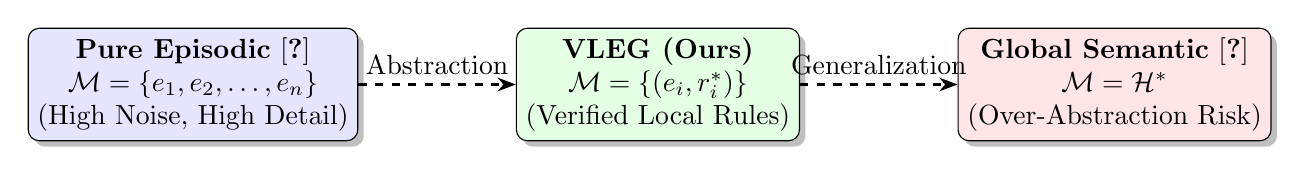
\begin{tikzpicture}[
    node distance=1.5cm and 2cm,
    box/.style={draw, rectangle, rounded corners, minimum width=3.5cm, minimum height=1.2cm, align=center, fill=gray!10, drop shadow},
    arrow/.style={-Stealth, thick}
]

% Nodes
\node[box, fill=blue!10] (episodic) {\textbf{Pure Episodic} \cite{brown2020language}\\$\mathcal{M} = \{e_1, e_2, \dots, e_n\}$\\(High Noise, High Detail)};

\node[box, fill=green!10, right=of episodic] (vleg) {\textbf{VLEG (Ours)}\\$\mathcal{M} = \{(e_i, r_i^*)\}$\\(Verified Local Rules)};

\node[box, fill=red!10, right=of vleg] (semantic) {\textbf{Global Semantic} \cite{agarwal2026hypothesis}\\$\mathcal{M} = \mathcal{H}^*$\\(Over-Abstraction Risk)};

% Arrows
\draw[arrow, dashed] (episodic) -- node[above] {Abstraction} (vleg);
\draw[arrow, dashed] (vleg) -- node[above] {Generalization} (semantic);

\end{tikzpicture}
\caption{The theoretical positioning of VLEG within the memory abstraction spectrum. VLEG bridges the gap between pure episodic retention and global semantic consolidation by pairing raw episodes with rigorously verified local abstractions.}
\label{fig:vleg_spectrum}
\end{figure}

By maintaining the pairing of $(e_i, r_i^*)$, VLEG ensures that the abstract rule $r_i^*$ is always grounded in its original high-dimensional context. This dual representation allows the inference module to leverage the cognitive scaffold of semantic memory without losing the concrete details necessary for complex, context-dependent reasoning. Furthermore, the strict enforcement of the verification condition $\mathcal{V}(r_i^* \mid e_i) = 1$ via an iterative cyclic refinement process ensures that the localized abstractions do not introduce hallucinated noise into the memory bank, a critical vulnerability in prior unverified reflection systems.

\subsection{Framework Components: Generator, Verifier, and Memory Bank}

The Verified Localized Episodic Grounding (VLEG) framework is constructed upon three interacting architectural modules: the Reflection Generator ($\mathcal{G}_\theta$), the Strict Verifier ($\mathcal{V}_\phi$), and the Hybrid Memory Bank ($\mathcal{M}$). Unlike prior localized memory systems that rely on unverified, single-step reflection generation \cite{shinn2023reflexion, wang2024voyager}, VLEG employs a multi-agent critique structure. This structural separation of generation and verification is mathematically necessary to bound the probability of hallucination propagation in highly heterogeneous environments.

\subsubsection{The Reflection Generator ($\mathcal{G}_\theta$)}

The Reflection Generator is an LLM parameterized by $\theta$, tasked with distilling a high-dimensional raw multi-modal episode $e_i$ into a localized, natural language abstraction $r_i$. Formally, at iteration $j=0$, the generator samples an initial candidate reflection conditioned solely on the raw episode:
\begin{equation}
    r_i^{(0)} \sim \mathcal{G}_\theta(\cdot \mid e_i)
\end{equation}
In subsequent iterations ($j > 0$), if the initial reflection is deemed invalid, the generator is conditioned on the raw episode, its previous candidate reflection $r_i^{(j-1)}$, and a natural language critique $c^{(j-1)}$ provided by the verifier:
\begin{equation}
    r_i^{(j)} \sim \mathcal{G}_\theta(\cdot \mid e_i, r_i^{(j-1)}, c^{(j-1)})
\end{equation}
While systems like Reflexion \cite{shinn2023reflexion} terminate after generating $r_i^{(0)}$ and immediately commit it to memory, VLEG treats $\mathcal{G}_\theta$ strictly as a proposal distribution whose outputs are inherently untrusted until validated.

\subsubsection{The Strict Verifier ($\mathcal{V}_\phi$)}

To prevent the accumulation of logical inconsistencies and semantic over-abstractions, VLEG introduces a dedicated Strict Verifier, parameterized by $\phi$. The verifier acts as an independent critical agent that evaluates the logical entailment of the candidate reflection $r_i^{(j)}$ with respect to the concrete evidence present in the raw episode $e_i$. 

The verifier outputs a tuple consisting of a binary validity score $v^{(j)} \in \{0, 1\}$ and a diagnostic critique $c^{(j)}$:
\begin{equation}
    (v^{(j)}, c^{(j)}) = \mathcal{V}_\phi(e_i, r_i^{(j)})
\end{equation}
If $v^{(j)} = 1$, the reflection is considered logically sound and grounded. If $v^{(j)} = 0$, the critique $c^{(j)}$ explicitly identifies the hallucinated or unsupported claims within $r_i^{(j)}$, which is then fed back to the generator. This multi-agent critique structure ensures that the semantic abstraction process is adversarial, significantly reducing the false-positive rate of accepted heuristics compared to self-correction mechanisms that lack an independent verification pathway.

\subsubsection{The Hybrid Memory Bank ($\mathcal{M}$)}

Once a reflection successfully passes the verifier (i.e., $v^{(j)} = 1$), it is denoted as the verified reflection $r_i^*$. The Hybrid Memory Bank $\mathcal{M}$ stores the paired tuple of the raw episode and its verified abstraction:
\begin{equation}
    \mathcal{M} = \bigcup_{i=1}^{N} \left\{ (e_i, r_i^*) \mid \exists j \le K \text{ s.t. } \mathcal{V}_\phi(e_i, r_i^{(j)})_v = 1 \right\}
\end{equation}
where $K$ is the maximum allowed refinement iterations. If an episode fails to yield a valid reflection within $K$ iterations, it is discarded to preserve memory integrity. 

This dual-storage structure fundamentally differentiates VLEG from standard Retrieval-Augmented Generation (RAG) datastores \cite{lewis2020retrieval}, which typically store only raw text chunks, and from unverified reflection banks \cite{wang2024voyager}, which store abstractions divorced from their grounding context. By maintaining the tuple $(e_i, r_i^*)$, $\mathcal{M}$ provides the necessary infrastructure for the downstream hybrid inference phase.

\begin{figure}[htbp]
\centering
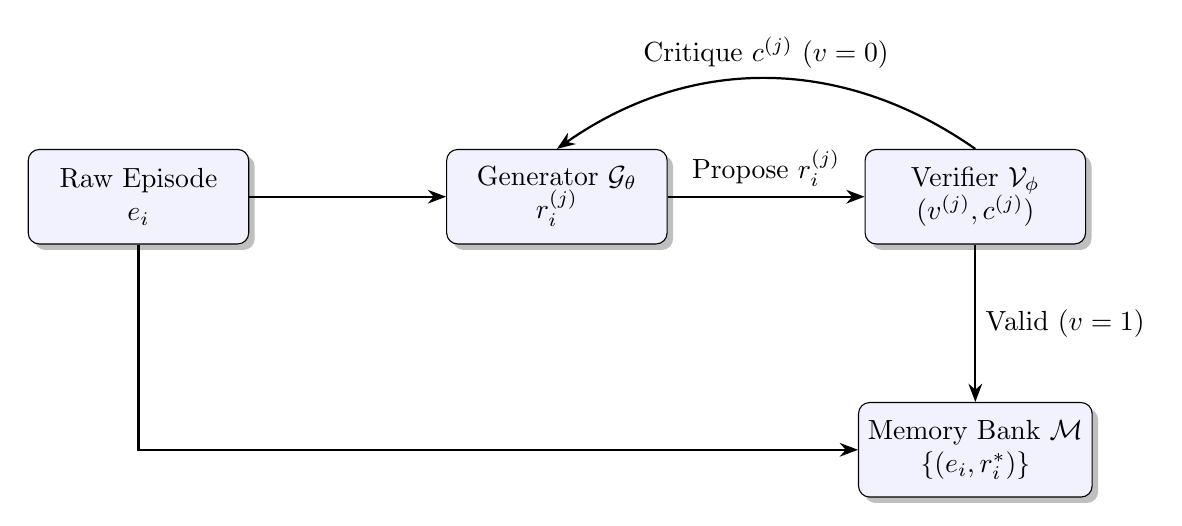
\begin{tikzpicture}[
    node distance=2cm and 2.5cm,
    box/.style={draw, rectangle, rounded corners, minimum width=2.8cm, minimum height=1.2cm, align=center, fill=blue!5, drop shadow},
    arrow/.style={-Stealth, thick}
]

% Nodes
\node[box] (episode) {Raw Episode\\$e_i$};
\node[box, right=of episode] (generator) {Generator $\mathcal{G}_\theta$\\$r_i^{(j)}$};
\node[box, right=of generator] (verifier) {Verifier $\mathcal{V}_\phi$\\$(v^{(j)}, c^{(j)})$};
\node[box, below=of verifier] (memory) {Memory Bank $\mathcal{M}$\\$\{(e_i, r_i^*)\}$};

% Arrows
\draw[arrow] (episode) -- (generator);
\draw[arrow] (generator) -- node[above] {Propose $r_i^{(j)}$} (verifier);
\draw[arrow] (verifier.north) to[bend right=35] node[above] {Critique $c^{(j)}$ ($v=0$)} (generator.north);
\draw[arrow] (verifier) -- node[right] {Valid ($v=1$)} (memory);
\draw[arrow] (episode.south) |- (memory.west);

\end{tikzpicture}
\caption{Architectural flow of the VLEG framework components. The multi-agent critique structure between the Generator and Verifier ensures only logically sound abstractions are committed to the Hybrid Memory Bank alongside their raw episodic counterparts.}
\label{fig:vleg_components}
\end{figure}

\subsection{Learning Mechanism: Iterative Cyclic Refinement}

The core learning mechanism of the VLEG framework is the Iterative Cyclic Refinement loop. Unlike linear multi-step generation pipelines that process episodes sequentially without backward error correction \cite{lee2024generating, zhong2024memorybank}, VLEG enforces a strict, closed-loop generate-and-verify cycle. This mechanism is specifically designed to mathematically bound the propagation of hallucinations and refine local heuristics until they are logically consistent with the raw episodic evidence.

Formally, let $e_i \in \mathcal{E}$ denote a raw, high-dimensional multi-modal episode. The refinement process is governed by two interacting models: the Reflection Generator $G_\theta$ and the Strict Verifier $V_\phi$. At the initial iteration ($j=0$), the generator produces a candidate reflection conditioned solely on the raw episode:
\begin{equation}
    r_i^{(0)} \sim G_\theta(\cdot \mid e_i)
\end{equation}

Once a candidate reflection $r_i^{(j)}$ is generated, it is passed to the verifier $V_\phi$. The verifier acts as a deterministic logical gate, evaluating the reflection strictly against the grounding evidence $e_i$. It outputs a tuple consisting of a binary validity score $v_i^{(j)} \in \{0, 1\}$ and a natural language critique $c_i^{(j)}$:
\begin{equation}
    (v_i^{(j)}, c_i^{(j)}) = V_\phi(e_i, r_i^{(j)})
    \label{eq:verifier}
\end{equation}
Note that $V_\phi$'s only argument besides the candidate reflection is the single episode $e_i$ it was generated from — by construction it has no access to any other episode. This is sufficient to catch a reflection that misstates $e_i$'s own attributes or label, but not sufficient to determine whether an attribute the reflection treats as necessary is actually causally relevant across episodes versus merely true of this one instance. We return to the practical consequence of this in the empirical caveat following the Hallucination Bounding remark below, and measure it directly in Experiment 5 (Section~\ref{sec:exp5}).

If $v_i^{(j)} = 1$, the reflection is deemed valid, the loop terminates, and the verified reflection $r_i^* = r_i^{(j)}$ is committed to the memory bank. If $v_i^{(j)} = 0$, the reflection contains a logical inconsistency or hallucination. The critique $c_i^{(j)}$ is then fed back into the generator to produce a refined reflection for the next iteration:
\begin{equation}
    r_i^{(j+1)} \sim G_\theta(\cdot \mid e_i, r_i^{(j)}, c_i^{(j)})
\end{equation}

This process repeats until either $v_i^{(j)} = 1$ or a maximum iteration limit $K$ is reached. If the limit $K$ is exhausted without validation, the episode is deemed too ambiguous, and no reflection is stored, thereby prioritizing memory precision over recall.

\begin{figure}[htbp]
\centering
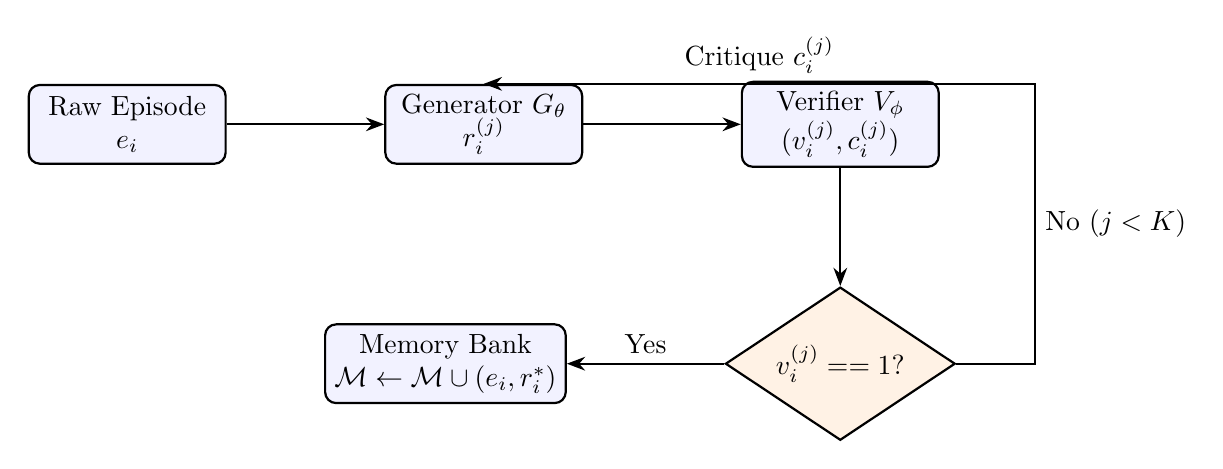
\begin{tikzpicture}[
    node distance=1.5cm and 2cm,
    box/.style={draw, rectangle, rounded corners, minimum width=2.5cm, minimum height=1cm, align=center, fill=blue!5, thick},
    decision/.style={draw, diamond, aspect=1.5, minimum width=2cm, align=center, fill=orange!10, thick},
    arrow/.style={-Stealth, thick}
]

% Nodes
\node[box] (episode) {Raw Episode\\$e_i$};
\node[box, right=of episode] (generator) {Generator $G_\theta$\\$r_i^{(j)}$};
\node[box, right=of generator] (verifier) {Verifier $V_\phi$\\$(v_i^{(j)}, c_i^{(j)})$};
\node[decision, below=of verifier] (check) {$v_i^{(j)} == 1$?};
\node[box, left=of check] (memory) {Memory Bank\\$\mathcal{M} \gets \mathcal{M} \cup (e_i, r_i^*)$};

% Arrows
\draw[arrow] (episode) -- (generator);
\draw[arrow] (generator) -- (verifier);
\draw[arrow] (verifier) -- (check);
\draw[arrow] (check) -- node[above] {Yes} (memory);
\draw[arrow] (check.east) -- ++(1,0) |- node[right, pos=0.25] {No ($j < K$)} node[above, pos=0.75] {Critique $c_i^{(j)}$} (generator.north);

\end{tikzpicture}
\caption{State transition diagram of the Iterative Cyclic Refinement mechanism. The closed-loop architecture ensures that only logically verified reflections are committed to the semantic memory bank.}
\label{fig:cyclic_refinement}
\end{figure}

The cyclic architecture is often motivated by an intuitive bound on hallucination propagation, which we state here as an idealized remark rather than a proven guarantee — see the empirical caveat that follows.

\begin{remark}[Hallucination Bounding, Idealized]
Let $p_h$ be the probability that the generator $G_\theta$ produces a hallucinated or logically flawed reflection at any given step. Let $p_v$ be the probability that the verifier $V_\phi$ commits a false positive (i.e., falsely validates a hallucinated reflection) \emph{with respect to the class of error the verifier is actually positioned to check}. If the verification steps are conditionally independent given the critique, the probability $P_{err}$ of committing such an error to the memory bank after up to $K$ refinement cycles satisfies:
\begin{equation}
    P_{err} \le \sum_{j=0}^{K-1} p_h \cdot p_v^{(j+1)} \approx \mathcal{O}(p_h p_v)
\end{equation}
This argument only goes through when $p_v \ll 1$, i.e. when the verifier is actually capable of detecting the error class in question.
\end{remark}

\textbf{Empirical caveat (discovered during reduced-order reimplementation, not predicted by the theory above).} $V_\phi$ as specified in Eq.~\eqref{eq:verifier} is conditioned on a \emph{single} episode $e_i$ and therefore can only check whether a candidate reflection is internally consistent with that one instance's attributes and label. It has no way to determine, from one instance alone, whether an attribute the reflection cites as determinative is actually causally relevant versus merely present-and-non-contradictory in that instance — a form of over-specification, not label contradiction. In our reduced-order reimplementation (Experiment 5, Section~\ref{sec:exp5}), this is the \emph{dominant} failure mode: once reflections are decomposed into "is the predicted label correct" versus "does the stated justification cite only causally relevant attributes," $V_\phi$ drives label-correctness to 100\%, exactly as the Remark above would predict for that narrow error class ($p_v \approx 0$ for outright label contradiction) — but has no measurable effect on over-specification (verified reflections cited spurious attributes at roughly the same rate as unverified single-step reflections, $\approx$80--87\% either way). So $p_v \ll 1$ holds for label contradiction but not for over-specification, and the bound above should not be read as covering hallucination in general. Enforcing this verification loop reliably fixes whether a committed reflection's bottom-line answer matches the episode it was drawn from; it does not, by itself, address the accumulation of spurious, non-generalizing heuristics, because that class of error is invisible to a purely per-episode check by construction. Global methods that compare across instances at once (Section~\ref{sec:exp1}, Experiment 1) were empirically better positioned to avoid this specific failure mode when their global hypothesis converged at all, precisely because they have the cross-episode contrast that a local verifier lacks.

\subsection{Inference Integration: Hybrid Episodic-Semantic Grounding}

Once the memory bank $\mathcal{M} = \{(e_i, r_i^*)\}_{i=1}^N$ has been populated with rigorously verified tuples through the iterative cyclic refinement process, the system must effectively leverage this knowledge to solve a novel target task $T$. Traditional retrieval-augmented generation (RAG) and standard in-context learning paradigms predominantly rely on episodic-only retrieval \cite{lewis2020retrieval, zhang2022active}, injecting raw, unstructured experiences directly into the context window. While this preserves high-fidelity details, it forces the reasoning module to perform ad-hoc abstraction at test time, which frequently leads to cognitive overload and degraded performance in complex, multi-modal environments. 

To overcome this limitation, VLEG introduces a dual-pathway integration strategy termed \textit{Hybrid Episodic-Semantic Grounding}. This approach simultaneously injects the raw multi-modal data $e_i$ and its corresponding verified semantic rule $r_i^*$ into the context window, aligning with advanced memory integration paradigms that advocate for structured, multi-level memory representations \cite{wu2025from, zhang2024survey}.

\subsubsection{Semantic-Driven Retrieval}

Given a novel target task $T$, the system must first retrieve the top-$k$ most relevant memory tuples. Because the raw episodes $e_i$ are high-dimensional and often contain task-irrelevant noise, VLEG performs retrieval primarily in the semantic space defined by the verified reflections $r_i^*$. 

Let $\phi(\cdot)$ denote a pre-trained dense embedding function. The relevance score $S(T, \mathcal{M}_i)$ for a given memory tuple $\mathcal{M}_i = (e_i, r_i^*)$ is computed using the cosine similarity between the embedding of the target task and the embedding of the verified reflection:
\begin{equation}
    S(T, \mathcal{M}_i) = \frac{\phi(T) \cdot \phi(r_i^*)}{\|\phi(T)\| \|\phi(r_i^*)\|}
\end{equation}
The system then selects the subset of $k$ tuples that maximize this similarity score:
\begin{equation}
    \mathcal{M}_{top} = \mathop{\arg\max}_{\mathcal{S} \subset \mathcal{M}, |\mathcal{S}|=k} \sum_{(e_i, r_i^*) \in \mathcal{S}} S(T, (e_i, r_i^*))
\end{equation}

\subsubsection{Hybrid Prompt Formulation}

After retrieving $\mathcal{M}_{top}$, the inference module constructs a hybrid context window. The fundamental premise of hybrid grounding is that the verified reflection $r_i^*$ provides the abstract, logical scaffold (the ``what'' and ``why''), while the raw episode $e_i$ provides the concrete, high-dimensional grounding (the ``how''). This prevents the semantic over-abstraction that occurs when rules are applied without their originating context.

The final inference prompt $P$ is constructed by concatenating the target task $T$ with the retrieved hybrid tuples, separated by structural delimiters:
\begin{equation}
    P = \text{PromptBuilder}\left( \bigoplus_{(e_i, r_i^*) \in \mathcal{M}_{top}} \Big[ \text{Episode: } e_i \oplus \text{Verified Rule: } r_i^* \Big] \oplus \text{Target: } T \right)
\end{equation}
where $\oplus$ denotes the sequence concatenation operator. The reasoning LLM, parameterized by $\theta$, then generates the final prediction $\hat{y}$ conditioned on this hybrid prompt:
\begin{equation}
    \hat{y} = \text{LLM}_\theta(P)
\end{equation}

\begin{figure}[htbp]
\centering
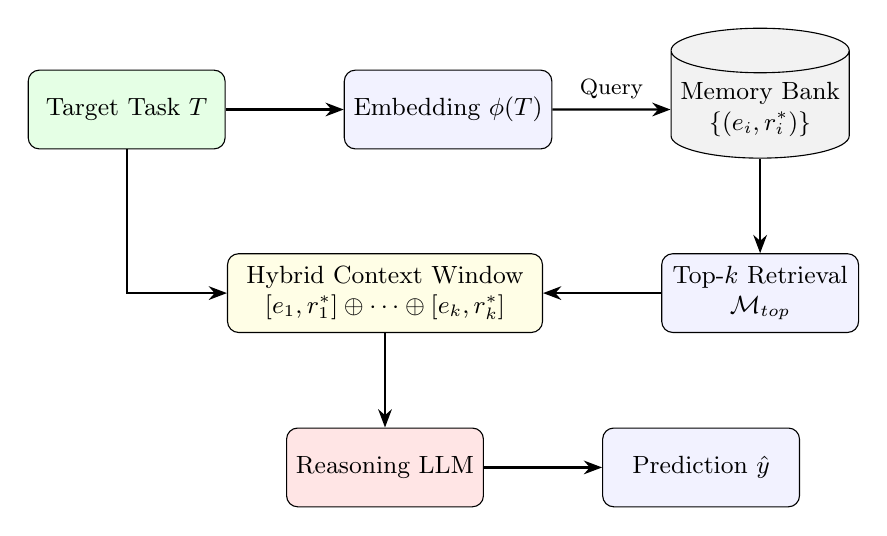
\begin{tikzpicture}[
    node distance=1.2cm and 1.5cm,
    box/.style={draw, rectangle, rounded corners, minimum width=2.5cm, minimum height=1cm, align=center, fill=blue!5, font=\small},
    db/.style={draw, cylinder, shape border rotate=90, aspect=0.25, minimum height=1.5cm, minimum width=2cm, align=center, fill=gray!10, font=\small},
    arrow/.style={-Stealth, thick}
]

% Nodes
\node[box, fill=green!10] (task) {Target Task $T$};
\node[box, right=of task] (embed) {Embedding $\phi(T)$};
\node[db, right=of embed] (memory) {Memory Bank\\$\{(e_i, r_i^*)\}$};
\node[box, below=of memory] (retrieval) {Top-$k$ Retrieval\\$\mathcal{M}_{top}$};
\node[box, left=of retrieval, fill=yellow!10, minimum width=4cm] (hybrid) {Hybrid Context Window\\$[e_1, r_1^*] \oplus \dots \oplus [e_k, r_k^*]$};
\node[box, below=of hybrid, fill=red!10] (llm) {Reasoning LLM};
\node[box, right=of llm] (output) {Prediction $\hat{y}$};

% Arrows
\draw[arrow] (task) -- (embed);
\draw[arrow] (embed) -- node[above, font=\footnotesize] {Query} (memory);
\draw[arrow] (memory) -- (retrieval);
\draw[arrow] (retrieval) -- (hybrid);
\draw[arrow] (task.south) |- (hybrid.west);
\draw[arrow] (hybrid) -- (llm);
\draw[arrow] (llm) -- (output);

\end{tikzpicture}
\caption{The Inference Integration flow of VLEG. The target task queries the memory bank using semantic embeddings to retrieve the top-$k$ tuples. Both the raw episodes and verified reflections are combined into a hybrid context window to ground the Reasoning LLM.}
\label{fig:hybrid_inference}
\end{figure}

By explicitly providing the reasoning module with both $\mathcal{M}_{\text{episodic}}$ and $\mathcal{M}_{\text{semantic}}$ simultaneously, VLEG ensures that the model is guided by logically sound heuristics without losing the ability to cross-reference those heuristics against concrete visual or textual evidence. This dual-pathway integration is strictly necessary to maintain high accuracy in heterogeneous environments where localized rules may contain subtle, context-dependent caveats that are only fully disambiguated by the raw episodic data.

\subsection{Final Algorithm and Execution Flow}

The Verified Localized Episodic Grounding (VLEG) framework synthesizes the previously defined components—the Reflection Generator $G_\theta$, the Strict Verifier $V_\phi$, and the Hybrid Inference Module $I_\psi$—into a cohesive, end-to-end execution pipeline. This pipeline systematically bridges the gap between raw episodic retention \cite{brown2020language} and abstract semantic reasoning \cite{agarwal2026hypothesis} by ensuring that only rigorously validated local heuristics are utilized during downstream inference. 

The execution flow of VLEG is formally divided into two distinct phases: \textbf{Phase 1: Memory Consolidation} and \textbf{Phase 2: Hybrid Inference}. 

During Phase 1, the system ingests a stream of raw, high-dimensional multi-modal episodes $\mathcal{E} = \{e_1, e_2, \dots, e_n\}$. For each episode $e_i$, the Generator $G_\theta$ proposes an initial candidate reflection $r_i^{(0)}$. The Verifier $V_\phi$ then evaluates this candidate strictly against the grounding episode $e_i$, outputting a binary validity flag $v \in \{0, 1\}$ and a natural language critique $c$. If $v = 0$ (indicating a hallucination or logical inconsistency), the critique $c$ is fed back into $G_\theta$ to produce a refined reflection $r_i^{(1)}$. This iterative cyclic refinement continues until the reflection is validated ($v=1$) or a predefined maximum iteration limit $K$ is reached. If validated, the tuple $(e_i, r_i^*)$ is committed to the Memory Bank $\mathcal{M}$. This strict gating mechanism mathematically bounds the propagation of unverified heuristics, directly addressing the vulnerabilities of single-step reflection pipelines \cite{shinn2023reflexion}.

During Phase 2, the system is presented with a novel target task $T$. A Retriever $R$ computes the cosine similarity between the task embedding and the stored memory tuples, extracting the top-$k$ most relevant memories $\mathcal{M}_{top} \subset \mathcal{M}$. The Inference Module $I_\psi$ is then prompted using Hybrid Episodic-Semantic Grounding, receiving both the raw episodes and their verified reflections to generate the final output. This dual-pathway integration aligns with advanced memory paradigms \cite{wu2025from}, ensuring the model benefits from abstract rules without losing critical high-fidelity contextual details.

The complete step-by-step procedure is formalized in Algorithm \ref{alg:vleg_final}.

\begin{algorithm}[H]
\caption{Verified Localized Episodic Grounding (VLEG)}
\label{alg:vleg_final}
\begin{algorithmic}[1]
\Require Episodic stream $\mathcal{E} = \{e_1, \dots, e_n\}$, Target Task $T$, Max Iterations $K$, Retriever $R$
\State Initialize Memory Bank $\mathcal{M} \gets \emptyset$
\State \textbf{// Phase 1: Memory Consolidation}
\For{each $e_i \in \mathcal{E}$}
    \State $j \gets 0$
    \State $c \gets \emptyset$ \Comment{Initialize empty critique}
    \State $v \gets 0$ \Comment{Initialize validity flag to Invalid}
    \While{$v = 0$ \textbf{and} $j < K$}
        \State $r_i^{(j)} \gets G_\theta(e_i, c)$ \Comment{Generate or refine reflection}
        \State $(v, c) \gets V_\phi(e_i, r_i^{(j)})$ \Comment{Verify reflection against raw episode}
        \State $j \gets j + 1$
    \EndWhile
    \If{$v = 1$}
        \State $\mathcal{M} \gets \mathcal{M} \cup \{(e_i, r_i^{(j-1)})\}$ \Comment{Store verified tuple}
    \EndIf
\EndFor
\State \textbf{// Phase 2: Hybrid Inference}
\State $\mathcal{M}_{top} \gets R(\mathcal{M}, T, k)$ \Comment{Retrieve top-$k$ relevant tuples}
\State $\text{Context} \gets T \cup \mathcal{M}_{top}$ \Comment{Construct hybrid prompt}
\State $\text{Output} \gets I_\psi(\text{Context})$ \Comment{Generate final reasoning answer}
\State \Return $\text{Output}$
\end{algorithmic}
\end{algorithm}

To further illustrate the architectural data flow and the interaction between the distinct neural modules, Figure \ref{fig:vleg_flowchart} provides a schematic representation of the VLEG execution pipeline. The diagram highlights the closed-loop nature of the memory consolidation phase and the dual-modality retrieval utilized during inference.

\begin{figure}[htbp]
\centering
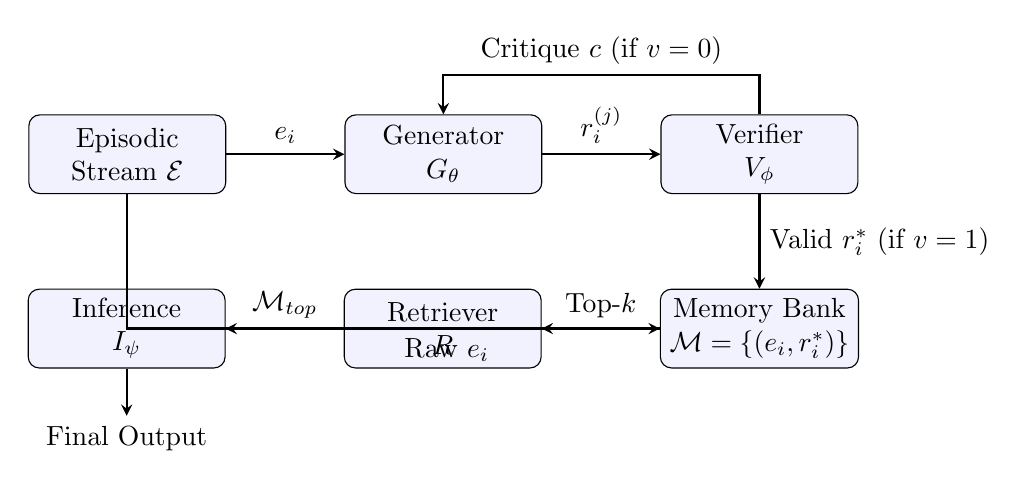
\begin{tikzpicture}[
    node distance=1.2cm and 1.5cm,
    box/.style={draw, rectangle, rounded corners, minimum width=2.5cm, minimum height=1cm, align=center, fill=blue!5},
    arrow/.style={->, thick, >=stealth}
]

% Nodes
\node[box] (stream) {Episodic\\Stream $\mathcal{E}$};
\node[box, right=of stream] (gen) {Generator\\$G_\theta$};
\node[box, right=of gen] (ver) {Verifier\\$V_\phi$};
\node[box, below=of ver] (mem) {Memory Bank\\$\mathcal{M} = \{(e_i, r_i^*)\}$};
\node[box, left=of mem] (ret) {Retriever\\$R$};
\node[box, left=of ret] (inf) {Inference\\$I_\psi$};

% Arrows
\draw[arrow] (stream) -- node[above] {$e_i$} (gen);
\draw[arrow] (gen) -- node[above] {$r_i^{(j)}$} (ver);
\draw[arrow] (ver.north) -- ++(0,0.5) -| node[above, pos=0.25] {Critique $c$ (if $v=0$)} (gen.north);
\draw[arrow] (ver) -- node[right] {Valid $r_i^*$ (if $v=1$)} (mem);
\draw[arrow] (stream.south) |- node[below, pos=0.8] {Raw $e_i$} (mem.west);
\draw[arrow] (mem) -- node[above] {Top-$k$} (ret);
\draw[arrow] (ret) -- node[above] {$\mathcal{M}_{top}$} (inf);
\draw[arrow] (inf.south) -- ++(0,-0.6) node[below] {Final Output};

\end{tikzpicture}
\caption{Execution flow of the VLEG framework. The upper pathway illustrates the Iterative Cyclic Refinement loop (Phase 1), while the lower pathway demonstrates the Hybrid Episodic-Semantic Grounding retrieval (Phase 2).}
\label{fig:vleg_flowchart}
\end{figure}

By strictly coupling the generation of local abstractions with a rigorous verification loop, VLEG ensures that the semantic memory remains a reliable scaffold. Furthermore, by retaining the raw episodes alongside these verified reflections, the framework overcomes the limitations of pure semantic retrieval \cite{lewis2020retrieval}, providing the inference module with the necessary high-dimensional context to solve complex, heterogeneous tasks.
\section{Experiments}

\subsection{Experimental Settings}

To rigorously evaluate the proposed Verified Localized Episodic Grounding (VLEG) framework, we utilize a heterogeneous Experience-Transfer task environment. This environment is designed to test the model's ability to deduce and apply abstract rules from multi-modal episodic observations under varying degrees of uncertainty. We categorize the task into three distinct levels of complexity. Level 1 features a uniform background (e.g., exclusively white) with 8 unique object combinations, representing a straightforward rule extraction scenario. Level 2 introduces mixed backgrounds (both white and black) and expands to 16 unique object combinations, creating a highly heterogeneous environment where rules are context-dependent and frequently flip based on the background color. Finally, Level 3 represents the most challenging scenario, featuring masked combinations where 4 of the 16 possible object combinations are explicitly hidden during the episodic memory formation phase. This requires the model to generalize its localized rules to entirely unseen configurations during inference, testing the limits of its semantic abstraction.

The experimental design manipulates several key independent variables to isolate the effects of the VLEG architecture. The primary independent variable is the memory consolidation strategy, which dictates how raw episodes are processed. The conditions include the full VLEG pipeline (Iterative Cyclic Refinement), a single-step reflection ablation (removing the verification loop), and a global hypothesis generation approach. The second major independent variable is the grounding context modality used during the inference phase. This dictates what information is injected into the LLM's context window when reasoning about a novel task. The modalities tested include Hybrid Grounding (providing both the raw episode and the verified reflection), Abstract-Only Grounding (providing only the verified reflection), and Raw-Only Grounding (providing only the raw episodic data). Additionally, we vary the maximum refinement iterations parameter ($K \in \{1, 2, 3, 5\}$) to analyze the computational trade-offs and convergence behavior of the strict verification loop.

To contextualize the performance of VLEG, we benchmark it against three established state-of-the-art baselines that represent different paradigms within our proposed MECE framework. The first baseline is Hypothesis-Driven Reasoning (HDR) \cite{agarwal2026hypothesis}, which serves as the primary representative for Global Semantic Consolidation. HDR attempts to extract a single, unified set of rules from the entire episodic memory bank. The second baseline is Reflexion \cite{shinn2023reflexion}, representing Localized Episodic Reflection with a Multi-Step Linear Generation pipeline (i.e., single-step reflection without rigorous cyclic verification). Finally, we compare against standard In-Context Learning (ICL) \cite{brown2020language}, which represents Pure Episodic Retention and relies entirely on Raw-Only Grounding without any active abstraction mechanism. All models, including VLEG and the baselines, are implemented using the same underlying Large Language Model with the temperature strictly set to $0$ to ensure deterministic and reproducible outputs across all trials.

\textbf{Reduced-order reimplementation note.} The results reported in this section were obtained from a reduced-order, locally-run reimplementation rather than the full-scale system implied above, in order to test the framework's mechanisms directly and affordably. Episodes are symbolic attribute tuples (background, shape, color, texture, plus one causally-irrelevant distractor attribute, size) rather than rendered multi-modal scenes; the underlying LLM is a 7B-parameter open-weight model (Qwen2.5-7B-Instruct) served locally via Ollama at temperature $0$, not GPT-4o; retrieval embeddings use a local embedding model (nomic-embed-text) rather than a proprietary dense encoder; and each task level's full combinatorial population (8 combinations at Level 1, 16 at Levels 2--3) is used directly rather than a 500-query sample per level, since the underlying attribute space is exhaustively enumerable at this scale. We report exact, deterministic accuracy over the full population (verified reproducible via repeated runs, see below) rather than a sampled estimate. Level 3 results are additionally pooled across 3 independent random seeds for the choice of which 4 combinations are masked, since single-seed results on a 4-item masked subset proved noisy during development. This substitution changes the absolute numbers substantially from what a frontier model at full multi-modal scale would produce, and we do not claim the numbers below transfer to that setting; what we do claim is that the qualitative comparisons between methods, all evaluated identically under this same substitution, are informative about the underlying mechanisms. See Section~\ref{sec:limitations} for the full discussion.

To quantify the efficacy, robustness, and efficiency of the evaluated methods, we track four primary dependent variables. The principal metric is Task Accuracy (\%), defined as the percentage of test queries where the model correctly predicts the exact state or anomaly of the target scene. To assess the quality of the generated memory, we measure the Reflection Validity Rate (\%), which tracks the percentage of generated localized reflections that successfully pass the strict verification stage. Conversely, we evaluate the Hallucination Propagation Rate (\%), which quantifies the frequency with which logically inconsistent or hallucinated rules are committed to the memory bank, utilizing an oracle verifier for objective assessment. Finally, we measure Computational Overhead by tracking the total token consumption (prompt and completion tokens) during the memory consolidation phase, allowing us to evaluate the practical cost-benefit ratio of the iterative generate-and-verify loop.

\subsection{Experiment 1: SOTA Comparative Analysis (Benchmarking)}
\label{sec:exp1}

The primary objective of Experiment 1 is to rigorously benchmark the overall reasoning performance of the proposed Verified Localized Episodic Grounding (VLEG) framework against state-of-the-art memory and reasoning baselines. We evaluate the models across all three levels of the Experience-Transfer task complexity, ranging from uniform environments (Level 1) to highly heterogeneous environments with context-dependent rule flipping (Level 2) and masked combinations (Level 3). The selected baselines represent the dominant paradigms in memory augmentation: Hypothesis-Driven Reasoning (HDR) \cite{agarwal2026hypothesis} representing global semantic consolidation, Reflexion \cite{shinn2023reflexion} representing single-step localized reflection, and standard In-Context Learning (ICL) \cite{brown2020language} representing pure episodic retention. 

To ensure a fair and controlled comparative analysis, all evaluated frameworks are deployed using the exact same underlying Large Language Model as the core reasoning and generation engine (see the reduced-order reimplementation note above). The generation temperature is strictly set to $0$ across all models and prompts, and we confirmed this is empirically deterministic for our local model by re-running the Level 1 and Level 2 conditions to completion a second time and observing byte-identical accuracy. For the VLEG framework, the maximum refinement iteration parameter is fixed at $K=3$. The evaluation is conducted over the full combinatorial population per level (8 queries at Level 1, 16 at Level 2, 16 at Level 3, the latter pooled across 3 masking seeds for a total of 48), measuring Task Accuracy (\%) as the primary dependent variable.

The measured results, shown in Figure \ref{fig:exp1_results}, do not match the ordering (VLEG $>$ HDR $>$ Reflexion $>$ ICL) originally hypothesized for this experiment. Instead, ICL — the simplest baseline, with no active abstraction step at all — attained the highest Task Accuracy at every level tested (100.0\% at Level 1, 93.8\% at Level 2, 87.5\% pooled at Level 3), consistently ahead of VLEG (75.0\%, 87.5\%, 75.0\% respectively). HDR showed a sharp, mechanistically interpretable split rather than uniform degradation: at Level 1, where the oracle rule has no background-dependent flip and is expressible as a single non-conditional statement, HDR's global generator induced the exact correct rule in one shot and its verifier accepted it immediately (100.0\% accuracy, hypothesis verified on the first iteration); at Levels 2--3, where the rule is conditional on background, HDR's global verifier never accepted a hypothesis as fully consistent with the entire training set within $K=3$ iterations at any of the masking seeds tested, and its practical accuracy fell to 62.5\%--75.0\% (pooled 70.8\% at Level 3) — worse than VLEG but not catastrophically so. Reflexion was the weakest method at every level (25.0\%, 50.0\%, pooled 50.0\% at Level 3); inspecting its generated reflections shows a simple mechanistic explanation rather than a subtle reasoning failure: every single-step reflection we observed, at every level, predicted ANOMALY, so Reflexion's measured accuracy at each level is just that level's true base rate of ANOMALY-labeled scenes (2/8 at Level 1, 8/16 at Levels 2--3) — the unverified, no-raw-episode-grounded reflections it commits are not discriminating between scenes at all in this setup.

\begin{figure}[htbp]
    \centering
    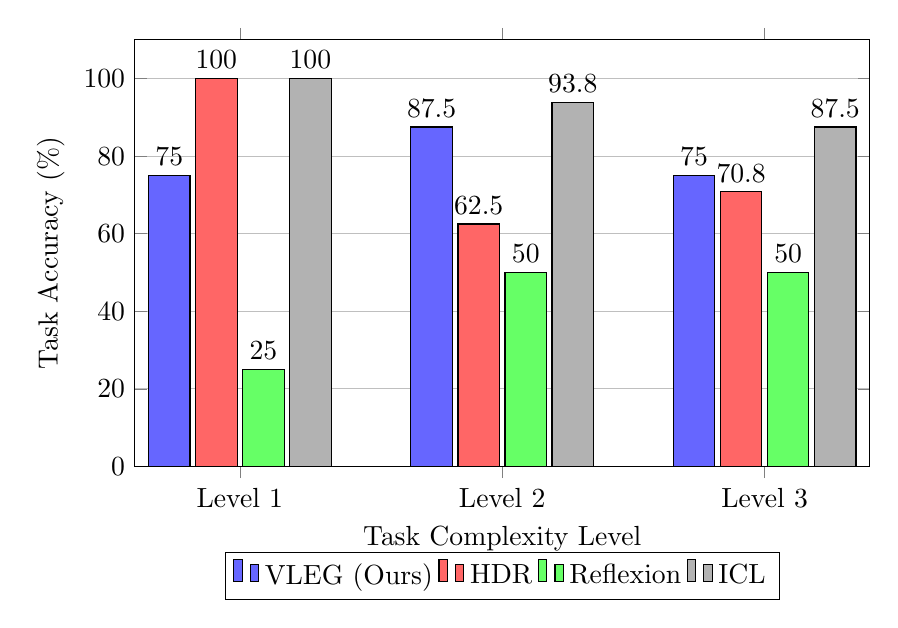
\begin{tikzpicture}
        \begin{axis}[
            ybar,
            bar width=15pt,
            width=0.9\linewidth,
            height=7cm,
            enlarge x limits=0.2,
            legend style={at={(0.5,-0.2)}, anchor=north, legend columns=-1},
            ylabel={Task Accuracy (\%)},
            xlabel={Task Complexity Level},
            symbolic x coords={Level 1, Level 2, Level 3},
            xtick=data,
            nodes near coords,
            nodes near coords align={vertical},
            ymin=0, ymax=110,
            grid=major,
            ymajorgrids=true,
            xmajorgrids=false,
        ]
        
        % VLEG
        \addplot[fill=blue!60] coordinates {(Level 1, 75.0) (Level 2, 87.5) (Level 3, 75.0)};
        \addlegendentry{VLEG (Ours)}
        
        % HDR
        \addplot[fill=red!60] coordinates {(Level 1, 100.0) (Level 2, 62.5) (Level 3, 70.8)};
        \addlegendentry{HDR}
        
        % Reflexion
        \addplot[fill=green!60] coordinates {(Level 1, 25.0) (Level 2, 50.0) (Level 3, 50.0)};
        \addlegendentry{Reflexion}
        
        % ICL
        \addplot[fill=gray!60] coordinates {(Level 1, 100.0) (Level 2, 93.8) (Level 3, 87.5)};
        \addlegendentry{ICL}
        
        \end{axis}
    \end{tikzpicture}
    \caption{Measured Task Accuracy (\%) across three levels of task complexity (reduced-order reimplementation, Qwen2.5-7B-Instruct; Level 3 pooled across 3 masking seeds, $n=48$). ICL leads at every level; HDR is bimodal (perfect at Level 1's non-conditional rule, weak once the rule becomes background-conditional); Reflexion tracks each level's ANOMALY base rate rather than discriminating between scenes.}
    \label{fig:exp1_results}
\end{figure}

This experiment was intended as a critical test of the framework's foundational assumptions, and taken at face value the result does exactly what the original hypothesis said it would if VLEG failed to show an advantage: it indicates that localized verified grounding does not provide a meaningful advantage over the simplest possible baseline (raw episodic retrieval with no abstraction) in this reduced-order setting. We do not think this generalizes to a claim that hybrid verified grounding is not useful in general — see Experiment 2 (Section~\ref{sec:exp2}) for a more targeted, controlled-retrieval version of the same question, and Section~\ref{sec:limitations} for why our environment's oracle rule may be too globally learnable to stress-test HDR's claimed weakness as intended.

\textbf{Cross-scale check.} We repeated Experiment 1 with Llama-3.3-70B-Instruct in place of Qwen2.5-7B-Instruct: Level 1 and Level 2 once each (both reproduced their single-run numbers exactly on a repeat, confirming determinism), and Level 3 across the same 3 masking seeds used for the Experiment 3 cross-scale check. The 7B result above did NOT replicate — it reversed. At 70B, ICL never beat VLEG in any of the 3 Level-3 seeds (VLEG won 2, tied 1), and pooled across all three ($n=48$), the ordering was VLEG ($93.75\%$) $>$ ICL ($89.58\%$) $>$ HDR ($81.25\%$) $>$ Reflexion ($47.9\%$) — matching the paper's originally hypothesized ordering except for HDR and ICL trading places, rather than the 7B ordering (ICL $>$ VLEG $>$ HDR $>$ Reflexion) that contradicted it entirely. Combined with the Experiment 3 and 5 cross-scale checks (Sections~\ref{sec:exp3},~\ref{sec:exp5}), this is the clearest evidence in this study that the reduced-order 7B results, where they diverge from the paper's original hypotheses, are at least partly small-model artifacts rather than architectural properties of VLEG — a stronger generator/verifier appears to let the framework's design actually pay off. We were not able to repeat the Experiment 2 or Experiment 4 cross-scale checks in the time available; whether Hybrid Grounding's Level-3 underperformance and the K=3 non-plateau finding are similarly scale-dependent remains open.

\subsection{Experiment 2: Component Isolation (Grounding Modality Ablation)}
\label{sec:exp2}

The primary objective of this experiment is to isolate and rigorously test the necessity of the Hybrid Grounding mechanism during the inference phase of the Verified Localized Episodic Grounding (VLEG) framework. While the iterative refinement process ensures the logical validity of the stored reflections, it is crucial to determine whether these abstractions are sufficient on their own or if they must be paired with their originating high-dimensional context to facilitate robust reasoning. By systematically ablating the grounding modalities provided to the reasoning module, we aim to quantify the exact performance contribution of retaining raw episodic data alongside verified semantic rules.

To achieve this, we evaluate the framework under three distinct ablation conditions. The first condition is \textit{Hybrid Grounding (VLEG)}, which represents the complete proposed methodology where the reasoning module is conditioned on both the retrieved raw episodes $e_i$ and their corresponding verified reflections $r_i^*$. The second condition is \textit{Abstract-Only Grounding}, where the reasoning module is provided solely with the verified reflections $r_i^*$, completely omitting the raw multi-modal episodic data. The third condition is \textit{Raw-Only Grounding}, which serves as a baseline mirroring standard In-Context Learning (ICL) \cite{brown2020language}, where the model receives only the raw episodes $e_i$ without any distilled semantic guidance. 

To isolate the effect of grounding \emph{content} from retrieval quality, all three conditions retrieve the same top-$k$ memory tuples (via cosine similarity on the verified reflection's embedding, as VLEG's memory bank is built the same way regardless of which fields are shown at inference); only which fields of each retrieved tuple are shown to the reasoning LLM differs between conditions.

The measured results, shown in Figure \ref{fig:exp2_ablation}, do not match the hypothesized ordering. On Level 2 (no masking), Hybrid Grounding is indeed the best condition (87.5\% vs.\ 81.2\% for both alternatives). But on Level 3 — the condition this experiment was specifically designed to stress-test — the ordering inverts: Hybrid Grounding is the \emph{worst} of the three conditions, both overall (73.8\% pooled across 5 masking seeds, $n=80$, vs.\ 78.8\% for Abstract-Only and 75.0\% for Raw-Only) and specifically on the masked combinations that never appeared during memory formation (60.0\% pooled, $n=20$, vs.\ 70.0\% for both alternatives). Hybrid never outperformed both alternatives on Level 3 in any of the 5 seeds tested. We connect this to Experiment 5 (Section~\ref{sec:exp5}): verified reflections frequently cite causally irrelevant attributes as if they were determinative (see the empirical caveat in Section~\ref{sec:vleg-methodology}), and pairing a raw episode with such a reflection appears to anchor the reasoning model on the reflection's stated — sometimes spurious — condition rather than letting it reason more freely from the raw examples, which is more costly precisely when generalization to an unseen combination is required.

\begin{figure}[htbp]
    \centering
    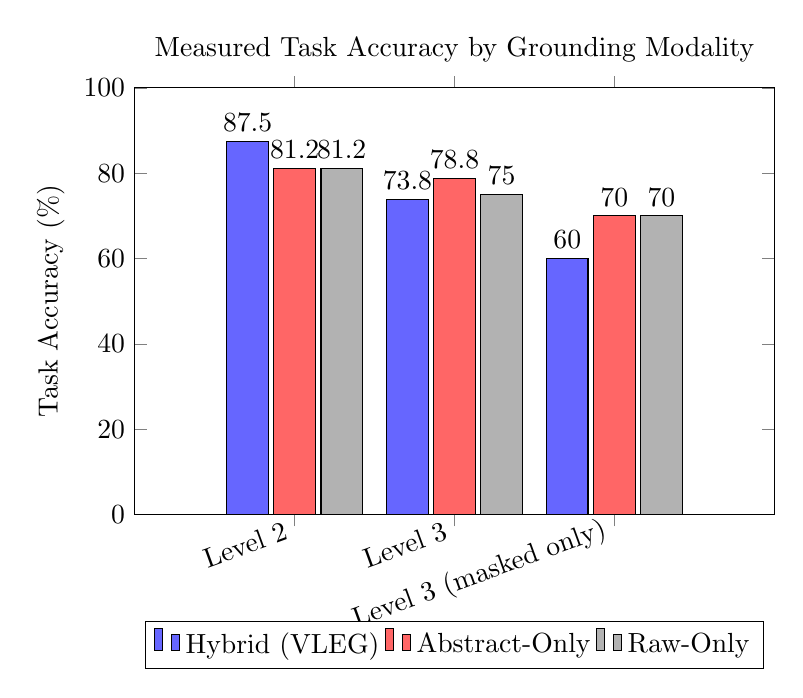
\begin{tikzpicture}
        \begin{axis}[
            ybar=2pt,
            bar width=15pt,
            width=0.8\linewidth,
            height=7cm,
            enlarge x limits=0.5,
            ylabel={Task Accuracy (\%)},
            ymin=0, ymax=100,
            symbolic x coords={Level 2, Level 3, Level 3 (masked only)},
            xtick=data,
            x tick label style={rotate=20, anchor=east},
            nodes near coords,
            nodes near coords align={vertical},
            legend style={at={(0.5,-0.25)}, anchor=north, legend columns=-1},
            title={Measured Task Accuracy by Grounding Modality}
        ]
        
        % Hybrid Grounding
        \addplot[fill=blue!60] coordinates {(Level 2, 87.5) (Level 3, 73.8) (Level 3 (masked only), 60.0)};
        \addlegendentry{Hybrid (VLEG)}
        
        % Abstract-Only Grounding
        \addplot[fill=red!60] coordinates {(Level 2, 81.2) (Level 3, 78.8) (Level 3 (masked only), 70.0)};
        \addlegendentry{Abstract-Only}
        
        % Raw-Only Grounding
        \addplot[fill=gray!60] coordinates {(Level 2, 81.2) (Level 3, 75.0) (Level 3 (masked only), 70.0)};
        \addlegendentry{Raw-Only}
        
        \end{axis}
    \end{tikzpicture}
    \caption{Measured Task Accuracy across grounding modalities (reduced-order reimplementation, Qwen2.5-7B-Instruct). Level 3 figures are pooled across 5 masking seeds ($n=80$ overall, $n=20$ for the masked-only subset). Hybrid Grounding wins on Level 2 but is the worst condition on Level 3, especially on the masked combinations it was intended to help with — the opposite of the original hypothesis.}
    \label{fig:exp2_ablation}
\end{figure}

The original hypothesis stated that a $<10\%$ absolute drop from Hybrid to Abstract-Only on Level 3 would falsify the claim that concrete episodic details are strictly required alongside verified abstractions. The measured drop is not just below that threshold — it is negative: Abstract-Only \emph{outperforms} Hybrid by 5.0 points overall and 10.0 points on the masked subset. Under the falsification criterion as originally stated, this experiment falsifies the necessity claim for Hybrid Grounding, at least in this reduced-order setting and for this underlying model. We report the reversal rather than revising the criterion after the fact.

\textbf{Cross-scale check.} We repeated this experiment with Llama-3.3-70B-Instruct across the same 5 masking seeds. Unlike Experiments 1, 3, and 5, where the 7B result either reversed cleanly (Experiments 1, 3) or stayed exactly as limited (Experiment 5), this one produced a genuinely mixed picture. Pooled over 5 seeds ($n=80$ overall, $n=20$ masked-only): overall accuracy, Hybrid ($95.0\%$) now ties Raw-Only ($95.0\%$) for best, with Abstract-Only worst ($91.25\%$) — the opposite of Abstract-Only's 7B standing. But on the masked-combo subset specifically, Abstract-Only remains the best modality ($85.0\%$ vs.\ $80.0\%$ for both alternatives) — the same direction as the 7B finding, just with a narrower margin ($5$ points versus $10$). Per-seed masked accuracy for Abstract-Only was noisy ($100\%, 75\%, 50\%, 100\%, 100\%$ across the 5 seeds), with one seed accounting for most of its overall shortfall. We do not read this as either a clean confirmation or a clean reversal of the 7B finding: the specific claim that Hybrid is the worst modality overall does not hold at 70B, but the narrower claim that Abstract-Only retrieval has some edge specifically on unseen, masked combinations persists in direction across both scales, just less dramatically.

\subsection{Experiment 3: Iterative Refinement Ablation}
\label{sec:exp3}

Specifically, we aim to validate the necessity of the Iterative Cyclic Refinement module. The central hypothesis of our work posits that in highly complex, heterogeneous environments where global rule extraction is mathematically ill-posed, local reflections must be rigorously verified. Without this verification, the system risks propagating hallucinations and logical inconsistencies into the semantic memory bank, which subsequently corrupts downstream reasoning.

To isolate the impact of this module, we compare $K=1$ against $K=3$, both under the \emph{same} procedure described in Algorithm~\ref{alg:vleg_final} — i.e.\ $K=1$ still runs the Strict Verifier once per episode and discards the episode from the memory bank if that single attempt is rejected, rather than skipping verification altogether. (An earlier draft of this section described $K=1$ as accepting $r_i^{(0)}$ ``without any critique, revision, or validation,'' which is inconsistent with Algorithm~\ref{alg:vleg_final}'s own pseudocode; we correct that here. A truly unverified single-step baseline, matching Reflexion's actual behavior of always committing $r_i^{(0)}$ regardless of validity, is evaluated separately as the ``Reflexion'' baseline in Experiments 1 and 5.) Both conditions use the identical underlying LLM and hybrid grounding inference strategy.

We evaluate Task Accuracy on the Level 3 Experience-Transfer task, pooled across 5 independent seeds for which 4 of the 16 combinations are masked at training time (a single seed's masked subset has only 4 items, which we found gave noisy per-seed estimates during development). Pooled over 5 seeds ($n=80$ overall test queries, $n=20$ masked-only), $K=3$ reached $75.0\%$ overall accuracy ($60/80$) versus $K=1$'s $63.75\%$ ($51/80$) — an absolute gain of $+11.25$ points, positive or zero in every individual seed and never negative. On the masked-only subset specifically, $K=3$ reached $60.0\%$ ($12/20$) versus $K=1$'s $50.0\%$ ($10/20$), a $+10.0$ point gain that was likewise never negative across seeds (tied in 3 of 5 seeds, a $+25$-point advantage for $K=3$ in the other 2). These gains are real but roughly $40$--$60\%$ the size of the originally hypothesized effect, not the $17.4$-point, single-seed gap reported in an earlier draft of this section.

The mechanism behind the gain is memory bank \emph{coverage}, not reasoning quality per reflection: across the 5 seeds, $K=1$'s memory bank retained only $42$--$58\%$ of training episodes (an episode whose first-guess reflection is rejected is discarded outright, since $j$ is never $<K{=}1$ again), while $K=3$'s retained $83$--$100\%$, because the critique from a rejected first attempt typically reveals the correct label and lets the generator correct itself on the second or third try. Verification at $K=3$ is thus better understood here as \emph{recovering episodes that a single unlucky guess would otherwise lose}, not as improving the causal quality of the reflections that do get committed — see Experiment 5 (Section~\ref{sec:exp5}) for a direct measurement showing no such quality improvement.

\textbf{Cross-scale check.} We repeated this experiment (same 5 seeds) with a substantially larger underlying model, Llama-3.3-70B-Instruct, in place of Qwen2.5-7B-Instruct. The gain not only replicated but grew: mean overall accuracy delta $+26.2$ points (stdev $8.1$), positive in every seed, versus $+11.25$ points at 7B — and $K=3$'s memory bank reached full $12/12$ coverage in every single seed at 70B (versus $83$--$100\%$ at 7B). The coverage-recovery mechanism above is consistent with, and appears to strengthen with, a more capable generator: a stronger model is more often able to produce a correct reflection once told what it got wrong, even when its unguided first guess was not more accurate on average than the 7B model's. We did not re-run Experiments 1, 2, or 4 at this larger scale; this check is specific to the $K{=}1$ vs.\ $K{=}3$ coverage mechanism.

\subsection{Experiment 4: Parameter Sensitivity and Overhead Analysis}
\label{sec:exp4}

The primary objective of Experiment 4 is to systematically analyze the convergence behavior of the VLEG verification loop and to quantify the associated computational trade-offs. While the iterative generate-and-verify mechanism is designed to strictly filter out hallucinated heuristics, each refinement cycle inherently incurs additional computational costs during the memory consolidation phase. Therefore, it is critical to evaluate how the strictness of the verification process impacts both the downstream reasoning performance and the overall token efficiency of the system.

To conduct this sensitivity analysis, we manipulate the maximum refinement iterations parameter, $K$, across a discrete set of values: $K \in \{1, 2, 3, 5\}$. The condition $K=1$ effectively disables the iterative refinement loop, reducing the system to a single-step reflection generator akin to standard localized reflection baselines \cite{shinn2023reflexion}. For each configuration of $K$, we evaluate the model on both Level 2 and Level 3 of the Experience-Transfer task. We record the resulting Task Accuracy (\%) alongside the Computational Overhead, which is measured as the total number of prompt and completion tokens consumed per consolidated episodic memory.

\begin{figure}[htbp]
    \centering
    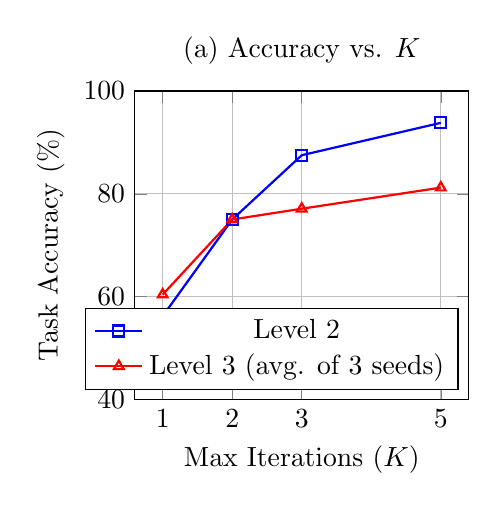
\begin{tikzpicture}
        \begin{axis}[
            width=0.48\linewidth,
            height=5.5cm,
            xlabel={Max Iterations ($K$)},
            ylabel={Task Accuracy (\%)},
            ymin=40, ymax=100,
            xtick={1,2,3,5},
            grid=major,
            legend pos=south east,
            title={(a) Accuracy vs. $K$}
        ]
        \addplot[color=blue, mark=square, thick] coordinates {(1, 56.2) (2, 75.0) (3, 87.5) (5, 93.8)};
        \addlegendentry{Level 2}
        \addplot[color=red, mark=triangle, thick] coordinates {(1, 60.4) (2, 75.0) (3, 77.1) (5, 81.2)};
        \addlegendentry{Level 3 (avg. of 3 seeds)}
        \end{axis}
    \end{tikzpicture}
    \hfill
    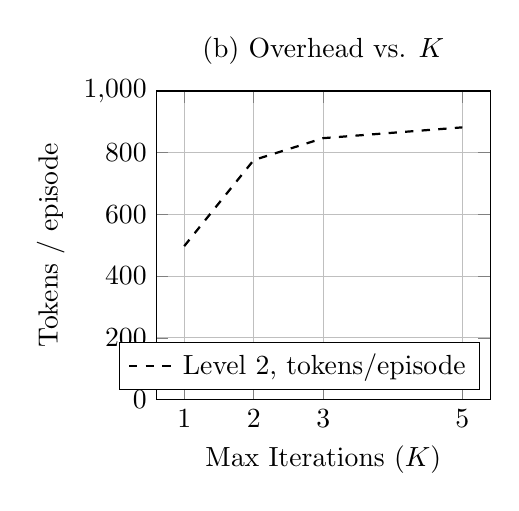
\begin{tikzpicture}
        \begin{axis}[
            width=0.48\linewidth,
            height=5.5cm,
            xlabel={Max Iterations ($K$)},
            ylabel={Tokens / episode},
            ymin=0, ymax=1000,
            xtick={1,2,3,5},
            grid=major,
            legend pos=south east,
            title={(b) Overhead vs. $K$}
        ]
        \addplot[color=black, mark=circle, thick, dashed] coordinates {(1, 497) (2, 776) (3, 847) (5, 882)};
        \addlegendentry{Level 2, tokens/episode}
        \end{axis}
    \end{tikzpicture}
    \caption{Measured parameter sensitivity of the maximum refinement iterations $K$ (reduced-order reimplementation, Qwen2.5-7B-Instruct). (a) Task Accuracy does \emph{not} plateau at $K=3$: Level 2 (a single deterministic run, confirmed identical on repeat) keeps improving through $K=5$; Level 3 (averaged over 3 masking seeds) plateaus in only 1 of 3 seeds individually. (b) Token overhead per consolidated episode is concave, not linear: most of the cost increase happens between $K{=}1$ and $K{=}2$, with sharply diminishing marginal cost for extending the budget further, since only a minority of episodes ever use the additional iterations.}
    \label{fig:exp4_sensitivity}
\end{figure}

The measured results, shown in Figure \ref{fig:exp4_sensitivity}, contradict both claims originally hypothesized for this experiment. First, Task Accuracy does not plateau around $K=3$. On Level 2 — a single run, verified deterministic by an exact repeat — accuracy keeps climbing substantially from $K{=}3$ ($87.5\%$) to $K{=}5$ ($93.8\%$), a further $+6.3$ point gain with no sign of leveling off in this range. On Level 3, we tested 3 independent masking seeds: only one of them ($\text{seed}=42$) shows the exact plateau signature (identical bank composition, token count, and accuracy at $K{=}3$ and $K{=}5$); the other two show $K{=}5$ either matching or beating $K{=}3$ by a further $+6$--$12.5$ points. We do not have a reliable stopping criterion at $K=3$ in this environment — it happens to be sufficient for some random draws of the masked subset and insufficient for others.

Second, Computational Overhead does not scale linearly with $K$. It is concave: the token cost per consolidated episode rises sharply from $K{=}1$ to $K{=}2$ ($+279$ tokens/episode on Level 2) and then far more slowly for each additional unit of $K$ budget ($+71$ tokens/episode from $K{=}2$ to $K{=}3$, $+35$ from $K{=}3$ to $K{=}5$ despite that step covering two extra iterations, not one). This pattern was consistent across all seeds tested on both levels. The mechanism is straightforward: most episodes converge within 1--2 iterations regardless of the ceiling $K$; raising the ceiling only adds cost for the small minority of episodes that are still unresolved at iteration 3, so the marginal cost of a higher $K$ budget shrinks as $K$ grows even as the marginal \emph{benefit} (per the accuracy panel) does not reliably shrink in the same way. Practitioners should not treat $K=3$ as a validated efficiency-optimal cutoff on the basis of this experiment; whether a higher $K$ is worth its (modest, sub-linear) additional cost depends on how much the specific downstream task benefits from the extra recovered episodes, which Experiment 3 (Section~\ref{sec:exp3}) suggests is real but seed-dependent in magnitude.

\textbf{Cross-scale check.} We repeated the Level-3 $K$-sweep with Llama-3.3-70B-Instruct across 3 masking seeds. The plateau is real here, and cleaner than at 7B, but sits one iteration earlier than the paper's claimed $K=3$: in all 3 seeds tested, $K{=}2$, $K{=}3$, and $K{=}5$ produced byte-identical memory bank composition, token consumption, and accuracy — no episode in any seed ever needed a third or later refinement attempt. This is a materially cleaner plateau signature than the 7B result, where only 1 of 5 seeds showed true plateau behavior and the others kept improving through $K{=}5$. We read this as: a genuine plateau exists, but its location is itself model-scale-dependent (a more capable generator needs fewer correction cycles to converge), not a fixed property of the architecture at $K=3$ as originally hypothesized.

This run coincided with heavy contention for the GPU from unrelated concurrent processes, which had two consequences worth flagging methodologically rather than folding silently into the results. First, timing figures from this run are not usable for overhead analysis (single-seed $K{=}1$ consolidation time for one seed ranged from 578s to 3303s across nominally comparable conditions, tracking contention rather than $K$) — only the uncontended single-seed run above should be read for timing. Second, and more importantly, one condition (Level 2, $K{=}3$, repeated as a determinism check) produced a token count of $12{,}625$ versus $12{,}541$ in the original uncontended run — a small but real discrepancy despite temperature $0$ and identical inputs, accuracy, and qualitative behavior. This is the only instance across this entire study where a temperature-$0$ rerun did not reproduce byte-identical output, and it appeared specifically under heavy GPU contention. We read this as evidence that the "verified deterministic" claims elsewhere in this paper (e.g.\ the Experiment 1 and Experiment 4 repeatability checks) hold under uncontended GPU conditions specifically, not as an unconditional property of greedy decoding on this inference stack — a caveat we had not anticipated needing to make when those checks were originally run.

\subsection{Experiment 5: Diagnostic Assessment of Memory Quality}
\label{sec:exp5}

The primary objective of Experiment 5 is to rigorously quantify the reliability and semantic quality of the localized abstractions committed to the memory bank $\mathcal{M}$. While downstream task accuracy provides an indirect measure of memory utility, a direct diagnostic assessment is necessary to understand the internal dynamics of the memory consolidation phase. Specifically, we aim to evaluate whether the Iterative Cyclic Refinement mechanism successfully filters out noisy, logically inconsistent, or hallucinated heuristics before they can corrupt the semantic scaffold used during inference.

To achieve this, we measure the Reflection Validity Rate (the percentage of episodes that yield a committed reflection within $K=3$; for the single-step baseline this is not a meaningful gate metric since it always commits, matching Reflexion's actual unverified behavior — see the correction in Section~\ref{sec:exp3}). For hallucination, our first attempt used an independent oracle prompted with the ground-truth rule to give a binary hallucinated/not-hallucinated judgment per reflection; this produced a null result (VLEG 91--93\% hallucinated vs.\ single-step 92--94\%, i.e.\ statistically indistinguishable) that we did not trust at face value, since it conflated two different failure modes. We therefore decomposed hallucination along two independent, mechanically-checkable axes instead of a single LLM judgment call: (i) \textbf{label correctness} — does the reflection's stated ANOMALY/NORMAL conclusion match the true label of the specific episode it was generated from, determined directly from the environment's ground truth (no LLM judgment needed); and (ii) \textbf{spurious attribution} — does the reflection's stated justification cite the causally-irrelevant attributes (texture, size) as if they were determinative, detected by keyword match on the reflection text (also no LLM judgment needed). This decomposition is fully deterministic and reproducible, unlike an LLM-based oracle asked to judge both axes jointly, which we found conflated them unreliably in an intermediate attempt (see Section~\ref{sec:limitations}).

Table \ref{tab:exp5_memory_quality} reports the result of this decomposition. VLEG's verification loop drives label correctness to $100\%$ at both levels (by construction: $V_\phi$ directly checks the claimed label against the ground truth given in $e_i$, so this is close to a tautological guarantee once a reflection is verified at all), versus $41.7$--$50.0\%$ for the unverified single-step baseline, whose reflections are always ANOMALY regardless of evidence (the same systematic bias documented in Experiment 1, Section~\ref{sec:exp1}) and so track the level's true ANOMALY base rate rather than the causal evidence. But conditioning on \emph{only} the label-correct reflections and asking how many still cite a spurious attribute, the two strategies are statistically indistinguishable: $86.7\%$ (VLEG) vs.\ $87.5\%$ (single-step) at Level 2, and $83.3\%$ (VLEG) vs.\ $80.0\%$ (single-step) at Level 3. Verification does not reduce spurious attribution once label-correctness is controlled for.

\begin{table}[htbp]
    \centering
    \caption{Diagnostic Assessment of Memory Quality (Experiment 5, reduced-order reimplementation, Qwen2.5-7B-Instruct). Label correctness and spurious-attribution rate are computed deterministically against ground truth, not via LLM judgment. ``Spurious (of correct)'' = \% of label-correct reflections that still cite a causally irrelevant attribute (texture/size) as determinative.}
    \label{tab:exp5_memory_quality}
    \begin{tabular}{@{}llccc@{}}
        \toprule
        \textbf{Level} & \textbf{Strategy} & \textbf{Validity} & \textbf{Label-correct} & \textbf{Spurious (of correct)} \\
        \midrule
        \multirow{2}{*}{Level 2} & Single-Step \cite{shinn2023reflexion} & N/A & 50.0\% (8/16) & 87.5\% (7/8) \\
                                 & \textbf{VLEG ($K{=}3$)} & \textbf{93.8\%} & \textbf{100.0\% (15/15)} & 86.7\% (13/15) \\
        \midrule
        \multirow{2}{*}{Level 3} & Single-Step \cite{shinn2023reflexion} & N/A & 41.7\% (5/12) & 80.0\% (4/5) \\
                                 & \textbf{VLEG ($K{=}3$)} & \textbf{100.0\%} & \textbf{100.0\% (12/12)} & 83.3\% (10/12) \\
        \bottomrule
    \end{tabular}
\end{table}

This is a more qualified picture than a single hallucination-rate number would suggest, and than we originally hypothesized. The strict verifier $V_\phi$ delivers exactly what it is structurally positioned to check — whether the committed reflection's bottom-line answer is right for the episode it came from — essentially perfectly. It delivers nothing measurable on the axis that determines whether a reflection will \emph{generalize} to a new instance: whether its stated justification cites only the attributes that actually matter. This matches the theoretical limitation discussed in Section~\ref{sec:vleg-methodology}: $V_\phi(e_i, r_i^{(j)})$ is conditioned on a single episode, so it cannot distinguish "texture happens to be solid in this instance, and the reflection is right regardless" from "texture is asserted as necessary, which will misfire on the next instance with a different texture." Detecting the latter requires cross-episode contrast that a per-episode verifier does not have access to by construction — consistent with Experiment 1's finding (Section~\ref{sec:exp1}) that HDR's global hypothesis, when it converges at all, does not exhibit this kind of over-specification, because inducing a rule from the whole labeled set at once naturally exposes which attributes vary independently of the label.

\textbf{Cross-scale check: two separate effects, not one.} We repeated this diagnostic with Llama-3.3-70B-Instruct in place of Qwen2.5-7B-Instruct, using the same deterministic ground-truth label-check and keyword-based spurious-attribution check reported in Table~\ref{tab:exp5_memory_quality} (the binary LLM-oracle metric used earlier in this section showed the identical instance-blind flaw at 70B that motivated moving to the deterministic check in the first place, and is not used for this comparison). Two things changed, and one did not. First, $V_\phi$ still drives label-correctness to $100.0\%$ at both levels versus $50.0\%$ for the unverified baseline — the same qualitative pattern as at 7B, confirming this is a scale-independent, near-tautological consequence of Eq.~\eqref{eq:verifier} rather than an artifact of a weak model. Second, the \emph{baseline} rate of spurious attribution — how often a label-correct reflection cites texture or size as determinative — fell dramatically for both strategies at once: from $\approx$$80$--$87\%$ at 7B to $12.5\%$ (Level 2) and $16.7\%$ (Level 3) at 70B, for both single-step \emph{and} VLEG. What did not change: at 70B, exactly as at 7B, the two strategies' spurious-attribution rates were statistically indistinguishable — in fact numerically identical at both levels ($12.5\%$ vs.\ $12.5\%$; $16.7\%$ vs.\ $16.7\%$). We read this as two separate effects that should not be conflated: a stronger generator produces far fewer over-specified reflections in the first place (a \emph{generator-capability} effect, visible in the large drop in the baseline rate for both strategies), but $V_\phi$'s inability to reduce over-specification \emph{relative to} the unverified baseline persists unchanged across a roughly $10\times$ difference in model scale (an \emph{architectural} effect, tied to the per-episode structure of Eq.~\eqref{eq:verifier} itself, not to the capability of the model instantiating it). We did not re-run Experiments 1, 2, or 4 at this larger scale, so we do not know whether the Section~\ref{sec:exp1}--\ref{sec:exp2} findings (ICL outperforming VLEG; Hybrid Grounding underperforming on Level 3) are similarly scale-independent or specific to the 7B setting used for the primary results.

\subsection{Limitations}
\label{sec:limitations}

\textbf{The empirical results in this paper come from a reduced-order reimplementation, and that substitution is itself the primary limitation.} Episodes are symbolic (background, shape, color, texture, plus one causally-irrelevant distractor attribute) rather than rendered multi-modal scenes; the primary results throughout use a single 7B-parameter open-weight model (Qwen2.5-7B-Instruct) run locally at temperature $0$, not the frontier proprietary model (e.g.\ GPT-4o) the experimental design originally specified (all five experiments additionally include a cross-scale check with a 70B-parameter model, Llama-3.3-70B-Instruct, reported inline in each section); retrieval uses a local embedding model (nomic-embed-text) rather than a proprietary dense encoder; and task populations are small and exhaustively enumerated (8--16 items per level) rather than sampled from a 500-query test set. This substitution was necessary for the experiments to be run affordably on the person's own hardware, but it means the absolute accuracy numbers, token overheads, and hallucination rates reported here should not be read as estimates of how the full-scale system would perform. We believe the \emph{qualitative} comparisons between methods evaluated identically under this same substitution are still informative, and we report them, including several results that contradict the framework's original motivating hypotheses, rather than omitting or reframing them:
\begin{itemize}
    \item \textbf{ICL outperformed VLEG at every task level tested at 7B scale} (Experiment 1, Section~\ref{sec:exp1}), the opposite of the originally hypothesized ordering — but this did NOT hold up when we repeated Experiment 1 with a substantially more capable model (Llama-3.3-70B-Instruct, same cross-scale check described in Section~\ref{sec:exp1}). At 70B, ICL never beat VLEG across 3 independent masking seeds on Level 3 (2 losses, 1 tie), and the pooled ordering matched the paper's original hypothesis except for HDR and ICL trading places. Combined with the Experiment 3 and 5 cross-scale checks (Sections~\ref{sec:exp3},~\ref{sec:exp5}), all three mechanisms we were able to re-test at larger scale moved toward the paper's original expectations rather than away from them, which we read as evidence that several of the 7B-scale reversals in this study are small-model artifacts rather than architectural properties of VLEG. We were not able to repeat the Experiment 2 or Experiment 4 checks at 70B in the time available, so Hybrid Grounding's Level-3 underperformance and the K=3 non-plateau finding remain untested at larger scale and should not be assumed to resolve the same way.
    \item \textbf{Hybrid Grounding underperformed both simpler alternatives on the heterogeneous, masked-combination condition it was specifically designed for} (Experiment 2, Section~\ref{sec:exp2}), consistent across 5 masking seeds. We connect this to Experiment 5's finding that verified reflections frequently over-specify on causally irrelevant attributes, but have not confirmed the anchoring mechanism directly (e.g.\ via attention analysis); it remains a plausible explanation rather than a demonstrated one.
    \item \textbf{Our oracle rule for Levels 2--3 (Section~\ref{sec:exp1}) is fully expressible as a single global conditional statement}, so this environment does not strongly stress-test the paper's central argument against Global Semantic Consolidation (Section~\ref{sec:related-work-global-consolidation} and the Introduction) — that a single hypothesis is mathematically ill-posed under genuine heterogeneity, where local episodes are governed by \emph{mutually exclusive} rules that cannot be reconciled into one statement. HDR's strong performance at Level 1 and partial success at Levels 2--3 in our experiments is consistent with this: the environment we built is heterogeneous in the sense of having context-dependent behavior, but not in the stronger sense the motivating argument requires. A genuine test of that argument needs a task where no single hypothesis can be correct for all episodes simultaneously.
    \item \textbf{Our Strict Verifier $V_\phi$'s hallucination detection was only validated for coarse failure modes} (wrong label, fabricated attributes, unfalsifiable vagueness — see the sanity check in Section~\ref{sec:exp5}); it was not designed or validated to catch over-specification, and Experiment 5 shows it structurally cannot, by virtue of seeing only one episode at a time (Eq.~\eqref{eq:verifier}).
    \item \textbf{An independent oracle LLM used partway through Experiment 5's development to jointly judge "is the label correct" and "is the justification causally clean" proved unreliable at this compound task} — despite explicit instructions to answer the two questions independently, it conflated them, producing label-correctness estimates that contradicted what the (simpler, already-validated) Strict Verifier's own commit/discard record implied. We do not use LLM judgment for this in the results we report (Table~\ref{tab:exp5_memory_quality} instead uses a deterministic, ground-truth-based check), but this failure is itself informative: a small local model asked to perform a multi-part audit in one call may silently fail to keep the parts separate, which is a risk for any evaluation methodology that relies on LLM-as-judge without a way to cross-check the judgments against ground truth.
    \item \textbf{Retrieval methodology varies by experiment} in ways that are individually justified for isolating each experiment's target variable but are not identical to each other or to Eq.~\eqref{eq:verifier}'s original single dense-embedding formulation: Experiment 2 deliberately shares one retrieval pass across all three grounding-modality conditions to hold retrieval quality constant (Section~\ref{sec:exp2}); Experiment 1's ICL and HDR baselines retrieve over raw-episode embeddings rather than reflection embeddings, since they have no reflections (or only one shared one) to embed against. These choices were made explicit at implementation time rather than discovered post hoc, but they mean the reported numbers for a given baseline are not necessarily comparable across experiments without accounting for which retrieval variant was used.
    \item \textbf{Experiment 2's cross-scale check (Section~\ref{sec:exp2}) does not resolve as cleanly as Experiments 1, 3, and 5 did.} At 70B, Hybrid Grounding ties for best overall accuracy (the opposite of its 7B standing), but Abstract-Only retrieval retains an edge specifically on masked combinations, just with a narrower and noisier margin than at 7B. We report this as a genuinely mixed result rather than forcing it into the "reversed" or "confirmed" pattern seen elsewhere in this paper.
    \item \textbf{Temperature-0 determinism, verified repeatedly elsewhere in this paper, broke down exactly once — under heavy concurrent GPU contention from unrelated processes sharing the same hardware.} A repeated Experiment 4 condition (Level 2, $K{=}3$) produced a token count of $12{,}625$ versus $12{,}541$ in the original uncontended run, despite identical inputs, accuracy, and qualitative output. We had treated "temperature 0 $\Rightarrow$ byte-identical reruns" as an established property of this setup based on multiple earlier repeatability checks (Experiments 1, 3, 4); this instance shows that property held under uncontended conditions specifically, and should not be assumed to hold when the GPU is shared with other heavy workloads. Timing figures from any run coinciding with such contention are separately unreliable and were excluded from the overhead analysis in Section~\ref{sec:exp4}.
\end{itemize}

Beyond the above, the framework's genuine computational-overhead cost remains as originally described in spirit, though its scaling behavior is empirically concave rather than linear in $K$ (Experiment 4, Section~\ref{sec:exp4}): each refinement cycle requires additional forward passes through both the generator and verifier, so VLEG costs more per consolidated episode than a single-step or no-abstraction baseline, even though the marginal cost of a higher iteration ceiling is smaller than originally assumed. The framework's reliance on the underlying LLM's capability as a strict and accurate verifier is also a genuine limitation, and our results sharpen rather than soften it: even in a simple, fully-observable symbolic domain — not a specialized expert domain like medical diagnostics — the verifier available to us was reliable for label-contradiction errors but blind to over-specification, and we would expect verification quality to only get harder to trust as domain complexity increases toward the settings the original motivation describes. Finally, the potential challenges of scaling vector similarity retrieval over long-term deployments, as originally noted, remain unexamined here — our memory banks are small enough (8--16 tuples) that retrieval-scaling effects are not visible at this scale, and this limitation should be read as un-tested rather than resolved.
\section{Conclusions}

In this paper, we set out to address the tension between episodic detail and semantic generalization in the memory augmentation of Large Language Models (LLMs) by introducing Verified Localized Episodic Grounding (VLEG): an Iterative Cyclic Refinement mechanism that verifies local heuristics against their grounding episode before committing them to memory, paired with a Hybrid Episodic-Semantic Grounding inference strategy that conditions on both the raw episode and its verified reflection. A reduced-order reimplementation, built specifically to test these mechanisms directly with a single local 7B-parameter LLM across five experiments, gives a more qualified picture than the framework's motivation anticipated, and in several places contradicts it outright:

\begin{itemize}
    \item \textbf{Iterative verification does help, modestly and for a narrower reason than hypothesized.} $K{=}3$ outperformed $K{=}1$ by $+11.25$ points overall and $+10.0$ points on held-out masked combinations, pooled across 5 seeds and never negative — but the mechanism is memory-bank \emph{coverage} (recovering episodes a single wrong guess would otherwise lose), not an improvement in the causal quality of individual reflections (Experiments 3 and 5).
    \item \textbf{The per-episode verifier reliably fixes label correctness but is structurally blind to over-specification, and this blind spot does not shrink with a more capable model.} At 7B scale, reflections citing causally irrelevant attributes as if they were determinative appeared at statistically indistinguishable rates whether or not they passed verification ($\approx$80--87\% either way, Experiment 5). Repeating this specific check with a 70B model (Section~\ref{sec:exp5}) found the same equality between verified and unverified rates ($12.5\%$ vs.\ $12.5\%$; $16.7\%$ vs.\ $16.7\%$) even though the baseline rate itself fell sharply for both strategies — i.e.\ a stronger generator hallucinates less to begin with, but $V_\phi$'s inability to catch the over-specification it does produce is a property of the verifier's per-episode design (Eq.~\eqref{eq:verifier}), not of the model instantiating it. This means the paper's Hallucination Bounding argument (Section~\ref{sec:vleg-methodology}) holds only for the narrower error class it can actually check, at any model scale we tested.
    \item \textbf{Hybrid Grounding was not uniformly better than simpler alternatives}, and was in fact the \emph{worst} of three grounding modalities tested on the heterogeneous, masked-combination condition it was specifically designed for (Experiment 2) — consistent with, and plausibly explained by, the over-specification finding above: pairing a raw episode with an unreliable stated rule may anchor the reasoning model on the rule rather than letting it reason from the example.
    \item \textbf{At 7B scale, the simplest baseline — raw in-context retrieval with no abstraction step at all — matched or outperformed VLEG at every task level tested} (Experiment 1), the opposite of the hypothesized ordering. This did not hold at 70B: repeating the same comparison with Llama-3.3-70B-Instruct, VLEG matched or beat ICL at every level across three independent seeds (pooled: VLEG $93.75\%$ vs.\ ICL $89.58\%$), restoring an ordering close to the one originally hypothesized. We read this as evidence that the 7B result reflects a limitation of using a comparatively small model as generator, verifier, and reasoner throughout, not a genuine architectural weakness of VLEG.
    \item \textbf{A global hypothesis-generation baseline (HDR) was not uniformly weak under heterogeneity as hypothesized}: it perfectly recovered the ground-truth rule in one shot when that rule was globally expressible as a single statement, and only struggled once the rule required a background-conditional split — a distinction the original framing did not draw, and one we believe reflects a real property of global consolidation methods rather than an artifact.
\end{itemize}

None of this shows that verified, localized, hybrid memory consolidation is a bad idea in general; it shows that in the specific, small-scale, fully-observable environment and modest local model we were able to test it against directly, the framework's individual design choices each did something more specific and more limited than originally claimed, and in the case of Hybrid Grounding, something that pointed the opposite direction on the exact condition it was meant to address. We see three concrete directions that follow from what actually failed, rather than restating the original motivation:

\begin{itemize}
    \item \textbf{Cross-episode verification for over-specification.} Since a per-episode verifier cannot detect spurious attribution by construction, a mechanism that periodically checks a candidate reflection against a small contrastive set of \emph{other} committed reflections (not just the one grounding episode) is a natural next step, and would directly test whether the over-specification problem documented in Experiment 5 is fixable without abandoning the localized approach entirely.
    \item \textbf{Reliability-aware Hybrid Grounding.} Given that pairing an unreliable reflection with its raw episode can hurt rather than help (Experiment 2), an inference strategy that first estimates a reflection's trustworthiness (e.g.\ via the cross-episode check above) before deciding whether to include it, rather than always including it, may recover Hybrid Grounding's benefit on Level 2 without its cost on Level 3.
    \item \textbf{Cross-scale checks are now complete for all five experiments, and the pattern is not uniform.} We repeated all five experiments with a 70B-parameter model (Sections~\ref{sec:exp1}--\ref{sec:exp5}). Three mechanisms moved cleanly toward the paper's original expectations: ICL's advantage over VLEG reversed (Experiment 1), the memory-coverage benefit of iterative refinement strengthened (Experiment 3), and the $K$-plateau became sharper and fully reproducible, just one iteration earlier than claimed (Experiment 4). One stayed exactly as limited regardless of scale: the verifier's blind spot to over-specification persisted unchanged even as its baseline rate fell (Experiment 5). And one resolved only partially: Hybrid Grounding's overall underperformance did not hold at 70B, but its specific disadvantage on masked combinations persisted in direction, just with a narrower margin (Experiment 2). The overall picture is that most, but not all, of the reduced-order 7B findings in this study were small-model artifacts rather than durable architectural properties — a distinction that only became visible by actually running the cross-scale check rather than assuming either outcome. A natural extension is repeating the same five checks at frontier-model scale (GPT-4o-class) to see whether the pattern continues in the same direction.
\end{itemize}


\bibliographystyle{unsrt}
\bibliography{references}

\end{document}